% This is samplepaper.tex, a sample chapter demonstrating the
% LLNCS macro package for Springer Computer Science proceedings;
% Version 2.21 of 2022/01/12
%
\documentclass[runningheads, 10pt]{llncs}
%
\usepackage[T1]{fontenc}
% T1 fonts will be used to generate the final print and online PDFs,
% so please use T1 fonts in your manuscript whenever possible.
% Other font encondings may result in incorrect characters.
%
\usepackage{caption}
\usepackage{subcaption}
\usepackage{graphicx} 
\usepackage{algorithm}
\usepackage{algorithmic}
\usepackage{amssymb}
\usepackage{mathtools}
\newcommand{\defeq}{\vcentcolon=}
\newcommand{\eqdef}{=\vcentcolon}
\usepackage{tikz} % nice language for creating drawings and diagrams
%\usepackage{tkz-graph}
\usetikzlibrary{positioning}
\usetikzlibrary{arrows}
\usetikzlibrary{arrows.meta}
\usepackage{pgfplots} % pack
% \let\doendproof\endproof
%\renewcommand\endproof{~\hfill\qed\doendproof}


% \usepackage{amsthm}
% \newtheorem{theorem}{Theorem}
% \newtheorem{corollary}{Corollary}[theorem]
% \newtheorem{lemma}[theorem]{Lemma}


\usepackage{graphicx}
% Used for displaying a sample figure. If possible, figure files should
% be included in EPS format.
%
% If you use the hyperref package, please uncomment the following two lines
% to display URLs in blue roman font according to Springer's eBook style:
% \usepackage{hyperref}
% \usepackage{color}
% \renewcommand\UrlFont{\color{blue}\rmfamily}
%
\begin{document}
%
\title{Fair Healthcare Rationing to Maximize Dynamic Utilities}
%
%\titlerunning{Abbreviated paper title}
% If the paper title is too long for the running head, you can set
% an abbreviated paper title here
%
\author{Aadityan Ganesh\inst{1}$^*$ \and
    Pratik Ghosal\inst{1}$^*$ \and
    Vishwa Prakash HV\inst{1}$^*$\and
    Prajakta Nimbhorkar\inst{1,2}$^*$}
% %
% \authorrunning{F. Author et al.}
% First names are abbreviated in the running head.
% If there are more than two authors, 'et al.' is used.
%
 \institute{Chennai Mathematical Institute, India \and
UMI ReLaX \\
\email{\{aadityanganesh,pratik,vishwa,prajakta\}@cmi.ac.in}}
%
\maketitle              % typeset the header of the contribution
%

\def\thefootnote{*}\footnotetext{The authors contributed equally to this work and are listed in alphabetical order}\def\thefootnote{\arabic{footnote}}


\begin{abstract}
Allocation of scarce healthcare resources under limited logistic and infrastructural facilities is a major issue in the modern society. We consider the problem of allocation of healthcare resources like vaccines to people or hospital beds to patients in an online manner. Our model takes into account the arrival of resources on a day-to-day basis, different categories of agents, the possible unavailability of agents on certain days, and the utility associated with each allotment as well as its variation over time. 

We propose a model where priorities for various categories are modelled in terms of utilities of agents.
We give online and offline algorithms to compute an allocation that respects eligibility of agents into different categories, and incentivizes agents not to hide their eligibility for some category. The offline algorithm gives an optimal allocation while the online algorithm gives an approximation to the optimal allocation in terms of total utility. Our algorithms are efficient, and maintain fairness among different categories of agents. Our models have applications in other areas like refugee settlement and visa allocation. We evaluate the performance of our algorithms on real-life and synthetic datasets. The experimental results show that the online algorithm is fast and performs better than the given theoretical bound in terms of total utility. Moreover, the experimental results confirm that our utility-based model correctly captures the priorities of categories.
\end{abstract}


\section{Introduction}


Recent years have witnessed the rise of human digitization~\cite{habermannDeepCapMonocularHuman2020,alexanderCREATINGPHOTOREALDIGITAL,pengNeuralBodyImplicit2021,alldieckDetailedHumanAvatars2018, rajANRArticulatedNeural2020}. This technology greatly impacts the entertainment, education, design, and engineering industry.
There is a well-developed industry solution for this task.
High-fidelity reconstruction of humans can be achieved either with full-body laser scans~\cite{saitoSCANimateWeaklySupervised2021}, dense synchronized multi-view cameras~\cite{xiangModelingClothingSeparate2021a,xiangDressingAvatarsDeep2022a}, or light stages~\cite{alexanderCREATINGPHOTOREALDIGITAL}.
However, these settings are expensive and tedious to deploy and consist of a complex processing pipeline, preventing the technology's democratization.

Another solution is to view the problem as inverse rendering and learn digital humans directly from custom-collected data.
Traditional approaches directly optimize explicit mesh representation~\cite{loperSMPLSkinnedMultiperson2015, fangRMPERegionalMultiperson2018, pavlakosExpressiveBodyCapture2019} which suffers from the problems of smooth geometry and coarse textures~\cite{prokudinSMPLpixNeuralAvatars2020,alldieckVideoBasedReconstruction2018}. Besides, they require professional artists to design human templates, rigging, and unwrapped UV coordinates.
Recently, with the help of volumetric-based implicit representations~\cite{mildenhallNeRFRepresentingScenes2020, parkDeepSDFLearningContinuous2019, meschederOccupancyNetworksLearning2019} and neural rendering~\cite{laineModularPrimitivesHighPerformance2020, liuSoftRasterizerDifferentiable2019, thiesDeferredNeuralRendering2019}, 
one can easily digitize a quality-plausible human avatar from video footage~\cite{jiangNeuManNeuralHuman2022,wengHumanNeRFFreeviewpointRendering}.
Particularly, volumetric-based implicit representations~\cite{mildenhallNeRFRepresentingScenes2020, pengNeuralBodyImplicit2021} can reconstruct scenes or objects with much higher fidelity against previous neural renderer~\cite{thiesDeferredNeuralRendering2019,prokudinSMPLpixNeuralAvatars2020}, and is more user-friendly as it does not need any human templates, pre-set rigging, or UV coordinates.
Captured visual footage and corresponding skeleton tracking are enough for training.
However, better reconstructions and more friendly usability are at the expense of the following factors.
1) \textbf{Inefficiency:}
They require longer optimization times (typically tens of hours or days) and inference slowly.
Volume rendering~\cite{mildenhallNeRFRepresentingScenes2020,lombardiNeuralVolumesLearning2019} formulates images by querying the densities and colors of millions of spatial coordinates. 
In the training stage, due to memory constraints, only a small fraction of points are sampled which leads to slow convergence speed.
2) \textbf{Entangled representations}:
The geometry, materials, and motion dynamics are entangled in the neural networks. 
Due to the implicit nature of neural nets, one can hardly edit one property without touching the others~\cite{yuanNeRFEditingGeometryEditing2022a,liuEditingConditionalRadiance2021}.
3) \textbf{Graphics incompatibility}:
Volume rendering is incompatible with the current popular graphic pipeline,
which renders triangular/quadrilateral meshes efficiently with the rasterization technique.
Many downstream applications require mesh rasterization in their workflow (\eg, editing~\cite{foundationBlenderOrgHome}, simulation~\cite{benderPositionBasedSimulationMethods2015}, real-time rendering~\cite{akenine2019real}, ray-tracing~\cite{waldRTXRayTracing}).
Although there are approaches~\cite{lorensenMarchingCubesHigh,labelleIsosurfaceStuffingFast2007} can convert volumetric fields into meshes, the gaps from discrete sampling degrade the output quality in terms of both meshes and textures.


To address these issues, we present \textbf{EMA}, a method based on \textbf{E}fficient \textbf{M}eshy neural fields to reconstruct animatable human \textbf{A}vatars.
Our method enjoys flexibility from implicit representations and efficiency from explicit meshes, yet still maintains high-fidelity reconstruction quality.
Given video sequences and the corresponding pose tracking, our method digitizes humans in terms of canonical triangular meshes, physically-based rendering (PBR) materials, and skinning weights \textit{w.r.t.} skeletons.
We jointly learn the above components via inverse rendering~\cite{laineModularPrimitivesHighPerformance2020,chenDIBRLearningPredict2021,chenLearningPredict3D2019} in an end-to-end manner.
Each of them is derived from a separate neural field, which relaxes the requirements of a preset human template, rigging, or UV coordinates.
Specifically, we predict a canonical mesh out of a signed distance field (SDF) by differentiable marching tetrahedra~\cite{shenDeepMarchingTetrahedra2021,gaoGET3DGenerativeModel,gaoLearningDeformableTetrahedral2020,munkbergExtractingTriangular3D2022}, then we extend the marching tetrahedra~\cite{shenDeepMarchingTetrahedra2021} for spatial-varying materials by utilizing a neural field to predict PBR materials \textit{on the mesh surfaces} after rasterization~\cite{munkbergExtractingTriangular3D2022,hasselgrenShapeLightMaterial2022,laineModularPrimitivesHighPerformance2020}.
To make the canonical mesh animatable, we take another neural field to model the forward linear blend skinning for the meshes. 
Given a posed skeleton, the canonical mesh is then transformed into the corresponding poses.
Finally, we shade the mesh with a rasterization-based differentiable renderer~\cite{laineModularPrimitivesHighPerformance2020} and train our models with a photo-metric loss.
After training, we export the mesh with materials and discard the neural fields.

\looseness=-1
There are several merits of our method design.
1) \textbf{Efficiency}:
Powered by efficient mesh rendering, our method can render in real-time.
Besides, the training speed is boosted as well, 
since we compute loss holistically on the whole image and the gradients only flow on the mesh surface. In contrast, volume rendering takes limited pixels for loss computation and back-propagates the gradients in the whole space.
Our method only needs about an hour of training and minutes of optimization are enough for plausible avatar reconstruction.
2) \textbf{Disentangled representations}:
Our shape, materials, and motion modules are disentangled naturally by design, which facilitates editing. 
Besides, Canonical meshes with forward skinning modeling handle the out-of-distribution poses better.
3) \textbf{Graphics compatibility}:
Our derived mesh representation is compatible with 
the prominent graphic pipeline, which leads to instant downstream applications (\eg, the shape and materials can be edited directly in design software~\cite{foundationBlenderOrgHome}).
To further improve reconstruction quality, we additionally optimize image-based environment lights and non-rigid motions.


We conduct extensive experiments on standards benchmarks H36M~\cite{ionescuHuman36MLarge2014b} and ZJU-MoCap~\cite{pengNeuralBodyImplicit2021}.
Our method achieves very competitive performance for novel view synthesis, generalizes better for novel poses, 
and significantly improves both training time and inference speed against previous arts.
Our research-oriented code reaches real-time inference speed (100+ FPS for rendering $512\times512$ images).
We in addition showcase applications including novel pose synthesis, material editing, and relighting.
\section{Optimal Offline Algorithm for Model $1$}\label{sec:offline-optimal-algorithm}

The problem can be modelled as an instance of the minimum cost flow network. We define the minimum cost flow problem here for completeness. 

\paragraph{The minimum cost flow problem:} The input is a flow network $G=(V,E)$ as a directed graph with node set $V$, edge set $E$, capacities $c_e>0$ and cost $u_e\in \mathbb{R}$ on each edge $e\in E$, and a source $s$ and sink $t$. A flow $f:E\rightarrow \mathbb{R}$ is a valid flow in $G$ if $f(e)\leq c(e)$, and the incoming flow at any node except $s$ and $t$ equals the outgoing flow. The cost of a flow $f(e)$ along an edge $e$ is
$u_e\cdot f(e)$. A minimum cost flow in the network is the one that minimizes the sum of costs of the flow along all edges.

There are polynomial-time algorithms known for the minimum cost flow problem. Also, it is known that if all the capacities are integers, then the optimum flow is an integer. We refer the reader to \cite{Ahuja93} for the details of minimum cost flow. 
\paragraph{Reduction: }
The construction of the flow network is shown in Figure~\ref{fig:flow-nw}. The flow network consists of a source $s$, a sink $t$, nodes for each day $d_j$, each agent $a_k$ and nodes $c_{ij}$ for each $(c_i,d_j)\in C\times D$. Each edge $(s,d_j)$ has capacity $s_j$ denoting the daily supply for day $d_j$, each edge $(d_j,c_{ij})$ has capacity equal to $q_{ij}$, and all other edges have capacity $1$. All the edges are directed. Additionally, each $(c_{ij},a_k)$ edge has cost $-u_k\cdot\delta_k^j$ whereas other edges have cost $0$.

\begin{proof}(of Theorem~\ref{thm:off-opt})
We show that a minimum cost flow $f$ in the flow network corresponds to a maximum utility matching in the given instance. The integrality of minimum cost flow implies that each edge incident on $t$ can have a flow of either $0$ or $1$. For each $k$, if $f(a_k,t)=1$, then 
there is exactly one $c_{ij}$ such that $f(c_{ij},a_k)=1$. Set $M(a_k)=(c_i,d_j)$ in the
corresponding matching $M$. Similarly, for any matching $M$, A corresponding flow  can be shown as follows. If $M(a_k)=(c_i,d_j)$ then set $f(a_k,t)=f(c_{ij},a_k)=1$, and set $f(s,d_j)$ equal to the number of agents vaccinated on day $d_j$, and $f(d_j,c_{ij})$ equal to the number of agents vaccinated on day $d_j$ through category $c_i$. It is clear that this is a valid flow in the network, and the negation of the cost of the flow is the same as the utility of the corresponding matching.
\end{proof}

\begin{figure}
  \centering
  \scalebox{1}{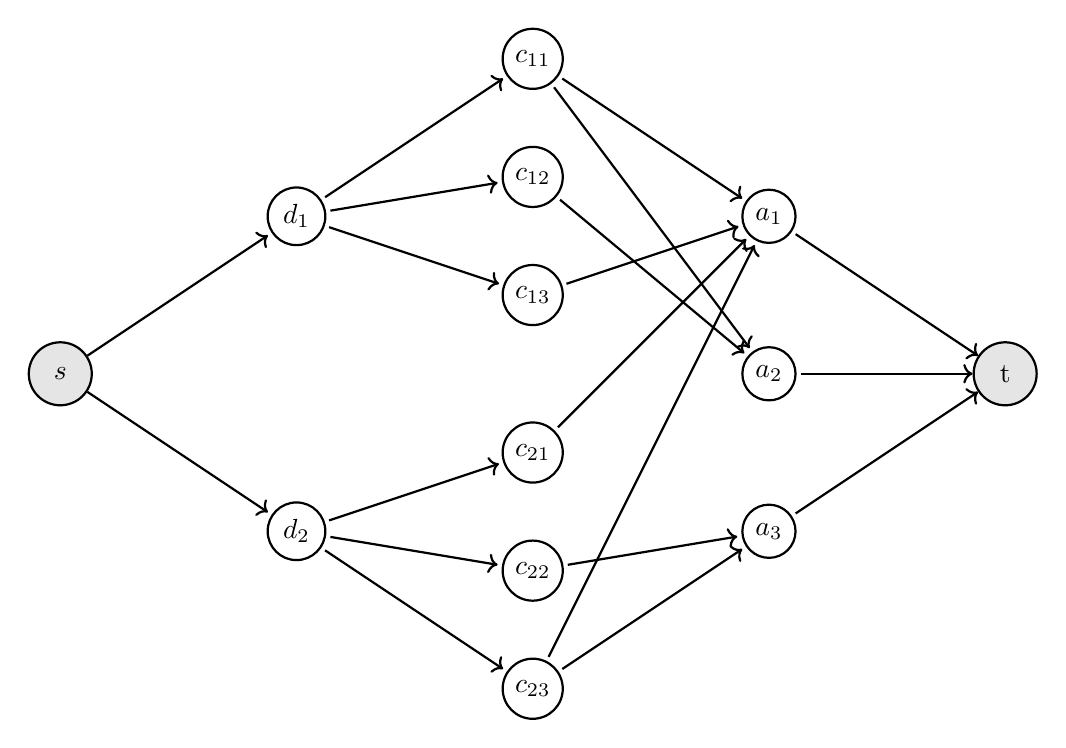
\begin{tikzpicture}[myn/.style={circle,thick,draw,inner sep=.1cm,outer sep=2pt},scale = 1,
      terminal/.style={circle, draw=black, fill=black!10, thick, minimum size=8mm},
      ]

      \node[terminal] (s) at (0,0) {$s$};
      \node[myn] (d1) at (3,2) {$d_1$};
      \node[myn] (d2) at (3,-2) {$d_2$};
      \node[myn] (c11) at (6,4) {$c_{11}$};
      \node[myn] (c12) at (6,2.5) {$c_{12}$};
      \node[myn] (c13) at (6,1) {$c_{13}$};
      \node[myn] (c21) at (6,-1) {$c_{21}$};
      \node[myn] (c22) at (6,-2.5) {$c_{22}$};
      \node[myn] (c23) at (6,-4) {$c_{23}$};
      \node[myn] (a1) at (9,2) {$a_1$};
      \node[myn] (a2) at (9,0) {$a_2$};
      \node[myn] (a3) at (9,-2) {$a_3$};
      \node[terminal] (t) at (12,0) {t};
      \draw[thick, ->] (s)--(d1);
      \draw[thick, ->] (s)--(d2);
      \draw[thick, ->] (d1)--(c11);
      \draw[thick, ->] (d1)--(c12);
      \draw[thick, ->] (d1)--(c13);
      \draw[thick, ->] (d2)--(c21);
      \draw[thick, ->] (d2)--(c22);
      \draw[thick, ->] (d2)--(c23);
      \draw[thick, ->] (c11)--(a1);
      \draw[thick, ->] (c13)--(a1);
      \draw[thick, ->] (c21)--(a1);
      \draw[thick, ->] (c23)--(a1);
      \draw[thick, ->] (c11)--(a2);
      \draw[thick, ->] (c12)--(a2);
      \draw[thick, ->] (c22)--(a3);
      \draw[thick, ->] (c23)--(a3);
      \draw[thick, ->] (a1)--(t);
      \draw[thick, ->] (a2)--(t);
      \draw[thick, ->] (a3)--(t);
    \end{tikzpicture}}
  \caption{Flow network for finding a maximum utility matching in Model 1}
\end{figure}\label{fig:flow-nw}
% note for self: a_1 is available on both days and belong to the first and third category. a_2 is available on day 1 and belongs to category 1 and 2. a3 is available only in category 2 and 3 and available on day 2 only

\section{Algorithms for Model~1}\label{sec:model1}
We give a flow based polynomial-time optimal offline algorithm for Model~1 in Appendix. Here, we give an online algorithm for the same which achieves a competitive ratio of \(1+\delta\), where \(\delta\) is the discounting factor of the agents.

\subsection{Online Algorithm for Model~1}
We present an online algorithm which greedily maximizes utility on each day. We show that this algorithm indeed achieves a competitive ratio of \(1+\delta\).\\

\emph{Outline of the Algorithm:} On each day \(d_i\), starting from day \(d_1\), we construct a bipartite graph \({H}_i=({A}_i\cup C, E_i, w_i)\) where \({A}_i\) is the set of agents who are available on day \(d_i\) and are not vaccinated  earlier than day $d_i$. 
%An edge $(a_j, c_k) \in E_i$ if $a_i$ is available on day $d_i$ and belongs to the category $c_k$.
Let the weight of the edge \((a_j, c_k) \in E_i\) be \(w_i(a_j, c_k) = \alpha_j.\delta^{i-1}\). We define capacity of the category $c _k \in C$ as  \(b'_{i,k}\). In this graph, our algorithm finds a maximum weighted b-matching of size not more than the daily supply value \(s_i\). 
% This can be found in polynomial time \cite{lawler2001combinatorial}. (Line 15 can be done in polytime)

\begin{algorithm}
  \caption{Online Algorithm for Vaccine Allocation}
  \label{alg:online-greedy-m1}
\textbf{Input:} An instance \(I\) of Model~1 \\
\textbf{Output:} A matching $M:A\to(C\times D)\cup\{\varnothing\}$ \\
\begin{algorithmic}[1] %[1] enables line numbers
    \STATE Let \(D,A,C\) be the set of Days, Agents and Categories respectively.
    \STATE \(M(a_j)\gets \varnothing\) for each $a_j \in A$
    \FOR {day \(d_i\) in \(D\)}
    \STATE \({A}_i \gets \{ a_j \in A \mid a_j\) is available on \(d_i\) and \(a_j\) is not vaccinated\}
    \STATE \(E_i\gets\{(a_j,c_k) \in {A}_i \times C \mid a_j\)is eligible to be vaccinated under category $c_k$ \}
    \FOR  {\((a_j,c_k)\) in \(E_i\)}
    \STATE Let \(w_i(a_j,c_k) \gets \alpha_j\delta^{i-1}\) 
    \ENDFOR
    \STATE Construct weighted bipartite graph \({H}_i=({A}_i\cup C, E_i,w_i)\).
    \FOR {\(c_k\) in \(C\)}
    \STATE \(b'_{i,k} \gets q_{ik}\) \COMMENT {Where \(q_{ik}\) is the daily quota}
    \ENDFOR
    \STATE Find maximum weight b-matching \(M_i\)  in \(H_i\) of size at most \(s_i\). \COMMENT{Where \(s_i\) is the daily supply}
    \FOR {each edge \((a_j,c_k)\) in \(M_i\)}
    \STATE \(M(a_j) \gets (c_k,d_i)\) \COMMENT{Mark \(a_j\) as vaccinated on day \(d_i\) under category \(c_k\)}
    \ENDFOR
    \ENDFOR\\
    \RETURN \(M\)
\end{algorithmic}
\end{algorithm}




The following lemma shows that the maximum weight b-matching computed in Algorithm~\ref{alg:online-greedy-m1} is also a maximum size b-matching of size at most \(s_i\). 

\begin{lemma}\label{lemma:max-size-max-wt}
  The maximum weight b-matching in \(H_i\) of size at most \(s_i\) is also a maximum size b-matching of size at most \(s_i\). 
\end{lemma}

\begin{proof}
  We prove that applying an augmenting path in \(H_i\) increases the weight of the matching. Consider a matching $M_i$ in $H_i$ such that \(M_i\) is not of maximum size and \(|M_i|<s_i\). Let $\rho = (a_1,c_1,a_2,c_2,\cdots,a_k,c_k)$ be an $M_i$-augmenting path in $H_i$. We know that every edge incident to an agent has the same weight in $H_i$. If we apply the augmenting path $\rho$, the weight of the matching increases by the weight of the edge \((a_1,c_1)\). This proves that a maximum weight matching in \(H_i\) of size at most $s_i$ is also a maximum size b-matching of size at most $s_i$.
\end{proof}



\subsection{Charging scheme}\label{sec:analysis-model-1}
We compare the solution obtained by Algorithm~\ref{alg:online-greedy-m1} with the optimal offline solution to get the worst-case competitive ratio for Algorithm~\ref{alg:online-greedy-m1}. Let $M$ be the output of Algorithm~\ref{alg:online-greedy-m1} and $N$ be an optimal offline solution. To compare $M$ and $N$, we devise a {\em charging scheme} by which, each agent $a_p$ matched in $N$ {\em charges} a unique agent $a_q$ matched in $M$. The amount charged, referred to as the {\em charging factor} here is the ratio of utilities obtained by matching $a_p$ and $a_q$ in $M$ and $N$ respectively.

Properties of the charging scheme:
\begin{enumerate}
\item Each agent matched in $N$ charges exactly one agent matched in $M$,
\item Each agent \(a_q\) matched in $M$ is charged by at most two agents matched in $N$, with charging factors at most $1$ and $\delta$. This implies that the utility of $N$ is at most $(1+\delta)$ times the utility of $M$.
\end{enumerate}

We divide the agents matched in $N$ into two types. Type $1$ agents are those which are matched in $M$ on an earlier day compared to that in $N$. Thus $a_p \in A$ is a Type $1$ agent if $a_p$ is matched on day $d_i$ in $M$ and on day $d_j$ in $N$, such that $i<j$. The remaining agents are called Type $2$ agents.
Our charging scheme is as follows:

\begin{enumerate}
\item Each Type~$1$ agent \(a_p\) charges themselves with a charging factor $\delta$, since the utility associated with them in $N$ is at most $\delta$ times that in $M$. 
  
\item Here onwards, we consider only Type $2$ agents and discuss the charging scheme associated with them.

  Let $X_i$ be the set of Type $2$ agents matched on day $d_i$ in $N$, and let $Y_i$ be the set of agents matched on day $d_i$ in $M$. Since Algorithm~\ref{alg:online-greedy-m1} greedily finds a maximum size b-matching of size at most \(s_i\), and as each edge in the b-matching corresponds to a unique agent, we show the following lemma holds:
\end{enumerate}
  \begin{lemma} For each \(d_i \in D\),  the set \(|X_i| \le |Y_i|\).\end{lemma} 

\begin{proof}
  Since $X_i$ contains only Type $2$ agents matched in $N_i$, the agents in $X_i$ are not matched by $M$ until day $i-1$. Therefore $X_i \subseteq A_i$, where $A_i$ is defined in Algorithm~\ref{alg:online-greedy-m1}. 
  The daily quota and the daily supply available for computation of $N_i$ and $M_i$ is the same i.e. $q_{i,k}$, and $s_i$ respectively.
  %The  of categories  We know that the capacity of each category in Model~1 is precisely her daily quota. Therefore $N_i$ is a matching in $H_i$ of size at most $s_i$. Since 
  By construction, $M_i$ is a matching that matches maximum number of agents in $A_i$, up to an upper limit of $s_i$, $|X_i| \leq |Y_i|$. 
\end{proof}
  To obtain the desired competitive ratio we design an injective mapping according to which, each agent \(a_p\) in \(X_i\) can uniquely charge an agent \(a_q\) in \(Y_i\) such that \(\alpha_p \le \alpha_q\). The following lemma shows that such an injective mapping always exists.

  \begin{lemma}\label{lemma:injection-exists}
    There exists an injective mapping \(f:X_i\to Y_i\) such that if \(f(a_p) = a_q\), then \(\alpha_p \le \alpha_q\). 
  \end{lemma}

\begin{proof}
    Let $N_i$ and $M_i$ respectively be the restrictions of $N$ and $M$ to day $d_i$. We construct an auxiliary bipartite graph $G_i$ where $X_i\cup Y_i$ form one bipartition and categories form another bipartition. The edge set is $N_i\cup M_i$. Then we set the capacity of $c_k$ in $G_i$ to be $b_{i,k}=q_{i,k}$. 

    The charging scheme is as follows. Consider the symmetric difference $M_i\oplus N_i$. It is known that  $M_i\oplus N_i$ can be decomposed into edge disjoint paths and even cycles \cite{NasreR17}.
    
    Consider a component \(C\) which is an even cycle as shown in Fig~\ref{fig:cycle-charging}. Since each agent \(a_p\) in \(C\) has both \(M_i\) edge and \(N_i\) edge indecent on it, agent \(a_p\) in \(X_i\) charges her own image in \(Y_i\) with a charging factor of \(1\).

    \begin{figure}[h]
    \begin{subfigure}[b]{0.49\textwidth}
      \centering
      \scalebox{0.5}{
      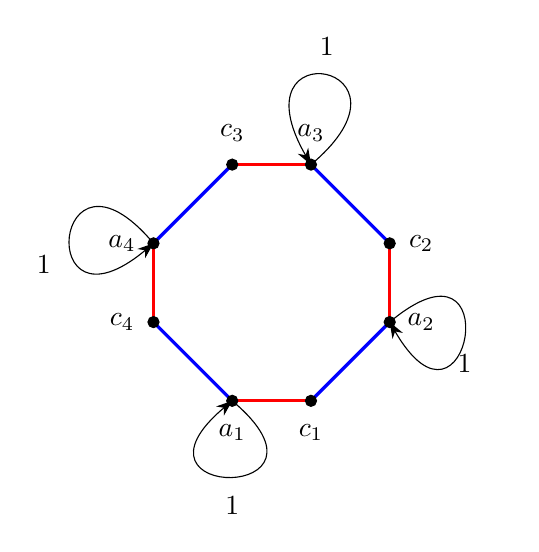
\begin{tikzpicture}[scale=1]
        
        %% vertex labels
        \node at (0,-0.4) {\(a_1\)};
        \node at (1,-0.4) {\(c_1\)};
        \node at (2.4,1) {\(a_2\)};
        \node at (2.4,2) {\(c_2\)};
        \node at (1,3.4) {\(a_3\)};
        \node at (0,3.4) {\(c_3\)};
        \node at (-1.4,2) {\(a_4\)};
        \node at (-1.4,1) {\(c_4\)};
        %%% edges
        \draw[very thick,red] (0,0) -- (1,0);
        \draw[very thick,red] (2,1) -- (2,2);
        \draw[very thick,red] (1,3) -- (0,3);
        \draw[very thick,red] (-1,2) -- (-1,1);

        \draw[very thick,blue] (1,0) -- (2,1);
        \draw[very thick,blue] (2,2) -- (1,3);
        \draw[very thick,blue] (0,3) -- (-1,2);
        \draw[very thick,blue] (-1,1) -- (0,0);

        \path[->,>={Stealth[scale=1.2]}, every loop/.style={min distance=2cm, looseness=40}, thin] (0,0)  edge  [in=-140,out=-40,loop] node [label=below:{1}] {} (0,0);
        
        \path[->,>={Stealth[scale=1.2]}, every loop/.style={min distance=2cm, looseness=40}, thin] (2,1)  edge  [in=-60,out=40,loop] node [label=below:{1}] {} (2,1);
        
        \path[->,>={Stealth[scale=1.2]}, every loop/.style={min distance=2cm, looseness=40}, thin] (1,3)  edge  [in=120,out=40,loop] node [label=above:{1}] {} (1,3);
        
        \path[->,>={Stealth[scale=1.2]}, every loop/.style={min distance=2cm, looseness=40}, thin] (-1,2)  edge  [in=-140,out=130,loop] node [label=below left:{1}] {} (-1,2);

        %% vertices
        \draw[fill=black] (0,0) circle (2pt);
        \draw[fill=black] (1,0) circle (2pt);
        \draw[fill=black] (2,1) circle (2pt);
        \draw[fill=black] (2,2) circle (2pt);
        \draw[fill=black] (1,3) circle (2pt);
        \draw[fill=black] (0,3) circle (2pt);
        \draw[fill=black] (-1,2) circle (2pt);
        \draw[fill=black] (-1,1) circle (2pt);

        
        % \end{scope}
      \end{tikzpicture}}
      \caption{Agents in cycles charge themselves with a charging factor or \(1\)}
      \label{fig:cycle-charging}
    \end{subfigure}
    \begin{subfigure}[b]{0.49\textwidth}
      \centering
      \scalebox{0.5}{
      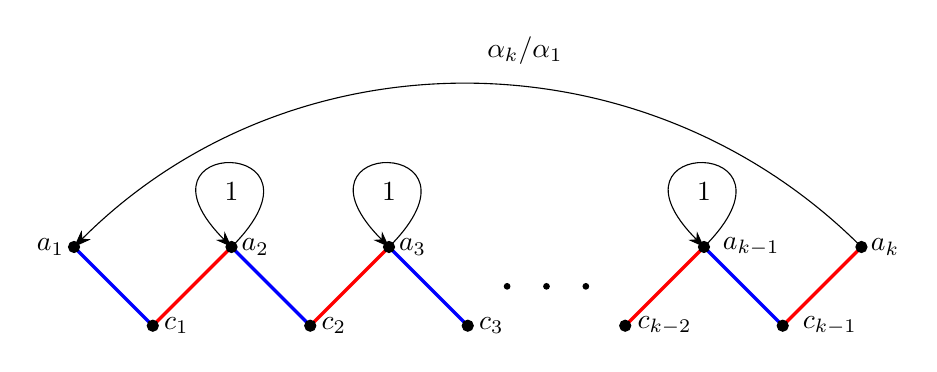
\begin{tikzpicture}
        
        %% vertex labels
        \node at (-1.3,1) {\(a_1\)};
        \node at (0.3,0) {\(c_1\)};
        \node at (1.3,1) {\(a_2\)};
        \node at (2.3,0) {\(c_2\)};
        \node at (3.3,1) {\(a_3\)};
        \node at (4.3,0) {\(c_3\)};

        \node at (6.5,0) {\(c_{k-2}\)};
        \node at (7.6,1) {\(a_{k-1}\)};
        \node at (8.6,0) {\(c_{k-1}\)};
        \node at (9.3,1) {\(a_k\)};
        %%% edges
        \draw[very thick,red] (0,0) -- (1,1);
        \draw[very thick,red] (2,0) -- (3,1);
        \draw[very thick,red] (6,0) -- (7,1);
        \draw[very thick,red] (8,0) -- (9,1);
        
        \draw[very thick,blue] (1,1) -- (2,0);
        \draw[very thick,blue] (0,0) -- (-1,1);
        \draw[very thick,blue] (3,1) -- (4,0);
        \draw[very thick,blue] (7,1) -- (8,0);

        \path[->,>={Stealth[scale=1.2]}, every loop/.style={min distance=2cm, looseness=40}, thin] (1,1)  edge  [in=135,out=45,loop] node [label=below:{1}] {} (1,1);
        \path[->,>={Stealth[scale=1.2]}, every loop/.style={min distance=2cm, looseness=40}, thin] (3,1)  edge  [in=135,out=45,loop] node [label=below:{1}] {} (3,1);
        \path[->,>={Stealth[scale=1.2]}, every loop/.style={min distance=2cm, looseness=40}, thin] (7,1)  edge  [in=135,out=45,loop] node [label=below:{1}] {} (7,1);

        \path[->,>={Stealth[scale=1.3]}, thin] (9,1)  edge  [in=45,out=135] node [label=above right:{\({\alpha_k}/{\alpha_1}\)}] {} (-1,1);

        %% vertices
        \draw[fill=black] (-1,1) circle (2pt);
        \draw[fill=black] (0,0) circle (2pt);
        \draw[fill=black] (1,1) circle (2pt);
        \draw[fill=black] (2,0) circle (2pt);
        \draw[fill=black] (3,1) circle (2pt);
        \draw[fill=black] (4,0) circle (2pt);
        \draw[fill=black] (4.5,0.5) circle (1pt);
        \draw[fill=black] (5,0.5) circle (1pt);
        \draw[fill=black] (5.5,0.5) circle (1pt);
        \draw[fill=black] (6,0) circle (2pt);
        \draw[fill=black] (7,1) circle (2pt);
        \draw[fill=black] (8,0) circle (2pt);
        \draw[fill=black] (9,1) circle (2pt);
        
      \end{tikzpicture}}
      \caption{Agents who are matched in both \(N_i\) and \(M_i\) charge themselves. Agent~\(a_k\) charges \(a_1\) with a factor or \({\alpha_k}/{\alpha_1}\). Red edges represent \(N_i\) and blue edges represent \(M_i\)}
      \label{fig:path-charging}
    
    \end{subfigure}
    \caption{Charging schemes}
    \end{figure}

    Now, Consider a component which is a path \(\rho\). There are two cases.
    
    \begin{enumerate}
    \item {\em Case 1: The path $\rho$ has an even length: }   If $\rho$ starts and ends at a category node, then each agent along the path is matched  in both \(N_i\) and \(M_i\). Hence, all such agents can charge themselves with a charging factor of \(1\).
    Suppose $\rho$ starts and ends at an agent as shown in Fig~\ref{fig:path-charging} i.e. \(\rho=(a_1,c_1,a_2,c_2,\cdots,a_{k-1},c_{k-1},a_k)\). Let \(a_1\) be matched in \(M_i\) and \(a_k\) is matched in \(N_i\). Then, \(\alpha_1\) must be greater than or equal to \(\alpha_k\). Otherwise from Lemma~\ref{lemma:max-size-max-wt}, \(M_i \oplus \rho\) is a matching of higher weight - which contradicts the fact that \(M_i\) is the maximum weight matching. Now, every agent in \(\rho\) except \(a_1\) and \(a_k\) charge themselves with a charging factor of \(1\) and \(a_k\) charges \(a_1\) with a charging factor of \({\alpha_k}/{\alpha_1}\).
    \item {\em Case 2: The path $\rho$ has an odd length:} Then either $\rho$ begins and ends with an $M_i$ edge or with an $N_i$ edge. If $\rho$ starts and ends with an $M_i$ edge, then every agent along the path who is matched in \(N_i\) is also matched in \(M_i\). Therefore all the agents on $\rho$ charge themselves.

Consider the case when $\rho$ starts with an \(N_i\) edge. Since $c_k$ is an end-point of $\rho$ with an $N_i$-edge, $c_k$ must have more agents matched to it in $N_i$ than that in $M_i$. So $c_k$ cannot be saturated in $M_i$.


%Now, depending on the saturation of $c_k$ in $M_i$ we have two subcases:
    
   % \emph{Subcase 1:} Suppose $c_k$ is saturated in $M_i$. That is, the number of \(M_i\) edges incident on \(c_k\) is equal to its capacity \(b_{i,k}\). But we know that the number of \(N_i\) edges incident on \(c_k\) is at most \(b_{i,k}\). This contradicts the fact that $c_k$ is an end-point of a path in $M_i \oplus N_i$. Therefore \emph{subcase 1} is not possible.
    As \(M_i\) is a maximum size matching [\ref{lemma:max-size-max-wt}], we cannot augment $M_i$ to $M_i\oplus \rho$ in $G_i$ even though both endpoints are unsaturated. This can happen only because the daily supply is met. That is $|M_i| = s_i$.  As $a_1$ is vaccinated in category $c_1$ in $N_i$, we claim that the weight $w(a_1, c_1)$ is less than every other edge in $M_i$. This is because if there exists an edge $e \in M_i$ such that $w(e) < w(a_1, c_1)$, we can remove the edge $e$ from $M_i$ and apply the augmenting path $\rho$ to get a matching with a higher weight, which is a contradiction. Therefore, as $w(a_1, c_1)$ is less than every other edge in \(M_i\), agent \(a_1\) can safely charge any agent \(a_q\) who is matched in \(M_i\). Since \(|M_i| \ge |N_i|\), we are guaranteed to have sufficient agents in \(N_i\) for charging.  
    \end{enumerate}
  \end{proof}
   

  % \item {\em Case 2: $|X_i|=|Y_i|+z, z>0$: } Let $N_i$ and $M_i$ respectively be the restrictions of $N$ and $M$ to day $d_i$. We construct an auxiliary bipartite graph $G_i$ where $X_i\cup Y_i$ form one bipartition and categories form another bipartition. The edge set is $N_i\cup M_i$. For a category $c_k$, let $n_{j,k}$ and $m_{j,k}$ be the number of agents matched in $N$ and $M$ respectively, under category $c_k$ on day $d_j$. Then we set the quota of $c_k$ in $G_i$ to be $b_{i,k}=\min\{q_{i,k}, \max\{q_k-\sum_{j=1}^{i-1}n_{j,k}, q_k-\sum_{j=1}^{i-1} m_{j,k}\}\}$. This is the maximum of the quotas of $c_k$ that were available for computation of $N_i$ and $M_i$ respectively.
  
  %   The charging scheme is given by the following. Consider the symmetric difference $M_i\oplus N_i$. Since $|N_i|=|M_i|+z$, there are exactly $z$ edge-disjoint alternating paths in $M_i\oplus N_i$ that start and end with an edge of $N$ \cite{NasreR17}. Let $\rho=\langle a_1,c_1,a_2,\ldots, a_k, c_k\rangle$ be one such path. Then $a_2,\ldots,a_{k-1}$ are matched in both $M_i$ and $N_i$, so they charge themselves with a charging factor of $1$. The agent $a_1$ charges $a_k$ with charging factor of $1$. It remains to decide whom $a_k$ charges.
  
  %   Since $\rho$ terminates at $c_k$ with an $N_i$-edge, the number of agents matched to $c_k$ in $N_i$ is more than those matched to $c_k$ in $M_i$. In Lemma~\ref{lem:saturated}, we show that this can happen only because of exhaustion of $q_k$ in Algorithm~\ref{alg:online-greedy-m2} on or before day $d_i$. %since $|M_i|, |N_i|\leq s_i$ and $M_i$ is a maximum matching on day $d_i$. 
  %   So agent $a_k$ can charge one of the agents matched to $c_k$ in $M$ on an earlier day, with charging factor $\delta$.


% \begin{lemma}\label{lem:saturated}
%   If node $c_k$ is an end-point of a path $\rho$ in $G_i$, then $q_k$ is exhausted in Algorithm \ref{alg:online-greedy-m2} on or before day $d_i$. 
% \end{lemma}
% \begin{proof}
%   Suppose $c_k$ be an endpoint of $\rho$ in $G_i$. The number of agents matched to $c_k$ in $N_i$ is more than those matched to $c_k$ in $M_i$. We know that the daily supply $s_i$ of the day $d_i$ is an upperbound for both $|M_i|$ and $|N_i|$. Since $|N_i| = |M_i| + z$, we have $|M_i| < s_i$. From Algorithm \ref{alg:online-greedy-m2} we know that $M_i$ is a maximum-size b-matching in $H_i$ of size at most \(s_i\). If the capacity of $c_k$ is not saturated in $H_i$, then we can augment the path $\rho$ contradicting the maximality of $M_i$.  Since $c_k$ has more edges of $M_i$ than $N_i$ incident to it, from the definition of $b_{i,k}$, category $c_k$ must have exhausted the overall quota $q_k$ in Algorithm \ref{alg:online-greedy-m2} on or before day $d_i$. 
% \end{proof}


% To show that Algorithm~\ref{alg:online-greedy-m1} achieves the desired competitive ratio, we introduce a \emph{charging scheme} - a mapping technique to compare the computed allocation with an optimal allocation. We say that an agent \(a_j\) who is vaccinated by an optimal allocation \emph{charges} an agent \(a_{j'}\) with a \emph{charging factor}. To be precise, we show that the set \(S_{OPT}\) of agents who are vaccinated by an optimal allocation can be partitioned into two parts \(H_1 \text{ and } H_2\) such that any agent \(a_{j'}\) who is vaccinated by the online allocation (computed by Algorithm~\ref{alg:online-greedy-m1}) is charged by at most one agent from each part. Furthermore, we show that each agent in \(H_1\) charges exactly one agent, with a charging factor of \(\delta_i\). And each agent \(a_j\) in \(H_2\) charges exactly one agent with a charging factor less than or equal to \(1\).

% Let \(ON\) be an allocation computed by Algorithm~\ref{alg:online-greedy-m1} on an instance \(I\), and let \(OPT\) be an optimal allocation on the same instance \(I\). Recall that an allocation \(M\) is of the form \(M:A\to(C\times D)\cup\{\varnothing\}\). Let \(S_{OPT}\) and \(S_{ON}\) be the sets of agents who got vaccinated by \(OPT\) and \(ON\) respectively. Now, \(H_1 \subseteq S_{OPT} \) can be described as the set of agents who are vaccinated by \(ON\) at least one day before they are vaccinated by \(OPT\) That is,
% \begin{align*}
%   H_1&=\{a\in S_{OPT} \mid OPT(a)=(c_i,d_j),\  ON(a)=(c_k,d_\ell), d_\ell<d_j\}
% \end{align*}

% For every agent \(a_i\in H_1\), \(a_i\) charges herself i.e. \(a_i \in S_{ON}\). Therefore, by definition, no two agents in \(H_1\) charge the same agent, and every agent in \(H_1\) charges exactly one agent in \(S_{ON}\). Since the utility associated with vaccinating $a_i$ in \(OPT\)is at most $\delta_i$ times that in \(ON\),the charging factor is $\delta_i$ in this case.

% Let \(S'_{OPT} = S_{OPT}\setminus H_1\). %be the remaining agents from \(S_{OPT}\) who are not in \(H_1\).

% To construct \(H_2\) and to introduce a charging scheme for \(H_2\), we first partition the agents in \(S'_{OPT}\) based on the day on which they got vaccinated by \(OPT\). That is, \[ S' = X_1\uplus X_2 \uplus \cdots \uplus X_{r=|D|} \]where,
% \begin{align*}
%   X_i &= \{a\in S' \mid a \text{ is vaccinated on day } d_i \text{ by } OPT  \} &&\forall {i\in\{1,2,\cdots,|D|\}}\\
% \end{align*}
% Similarly, let\[ S'_{ON} = Y_1\uplus Y_2 \uplus \cdots \uplus Y_{r=|D|} \] where,
% \begin{align*}
%   Y_i &= \{a\in S'_{ON} \mid a \text{ is vaccinated on day } d_i \text{ by } ON  \} &&\forall {i\in\{1,2,\cdots,|D|\}}\\
% \end{align*}

% Though Algorithm~\ref{alg:online-greedy-m1} finds maximum weight b-matching, the following lemma shows that the computed matching is also a maximum size matching.

% \begin{lemma}\label{lemma:max-size-max-wt}
%   The maximum weight b-matching in \((G_i,b^i_{ON})\) of size at most \(s_i\) is also a maximum size b-matching of size at most \(s_i\). 
% \end{lemma}
% \begin{proof}
%   We prove that applying a augmenting path increases the weight of that matching in \((G_i,b^i_{ON})\). Suppose $M_i$ be a matching of $(G_i, b^i_{ON})$ and $p$ be an $M_i$-augmenting path between the vertices $a$ and $c$ in $(G_i, b^i_{ON})$. We know that every edge incident to an agent has the same weight in $(G_i, b^i_{ON})$. When we apply the augmenting path $p$ the weight of the matching increases by the weight of the edge incident to $a$ in $p$. This proves that a maximum weight matching of \((G_i,b^i_{ON})\) of size at most $s_i$ is also a maximum size matching of \((G_i,b^i_{ON})\) of size at most $s_i$.
% \end{proof}

% Since Algorithm~\ref{alg:online-greedy-m1} greedily finds a maximum size b-matching of size at most \(s_i\), and since each edge in the b-matching corresponds to a unique agent, we note the following property
% \begin{remark} For each \(d_i \in D\),  the set \(|X_i| \le |Y_i|\).
% \end{remark}

% Now, we propose a charging scheme for the agents in the set \(H_2\). For each \(X_i\) and \(Y_i\), we give an injective mapping \(f\) from \(X_i\) to \(Y_i\) such that if \(f(a_i)=a_j\) then \(\delta_i\le \delta_j\).


% Now, it is apparent that an allocation by \(ON\) for \(A_i\) on day \(d_i\) is a valid matching in \((G_i,b^{ON}_i)\). Similarly, an allocation by \(OPT\) can be viewed as a matching in \((G_i,b^{OPT}_i)\). Let us call these matchings as \(M_i^{ON}\) and \(M_i^{OPT}\) respectively.
% \begin{align*}
%   M_i^{ON} &= \{(a_j,c_k) \mid a_j\in A_i \text{ is vaccinated on day } d_i \text{ under } c_k \text{ by } ON\}\\
%   M_i^{OPT} &= \{(a_j,c_k) \mid a_j\in A_i \text{ is vaccinated on day } d_i \text{ under } c_k \text{ by } OPT\}\\
% \end{align*}

% It is clear that \(|M_i^{OPT}| = |X_i|\) and \(|M_i^{ON}| = |Y_i|\).

% Let \(b_i:C \to \mathbb{Z}_{\ge 0}\) be defined as
% \begin{align*}
%   b_i(c_k) &= \max(b^{ON}_i(c_k), b^{OPT}_i(c_k))
% \end{align*}

% Clearly, both \(M_i^{OPT}\) and \(M_i^{ON}\) are valid b-matchings in \((G_i,b_i)\).

% Next we reduce the instance of a b-Matching problem to 1-matching \cite{gabow1983efficient}\cite{marsh1979matching} problem. Let \(G_i^{*}\) be the instance of $1$-matching problem corresponding to \((G_i,b_i)\). Both $N_i$ and $M_i$ are matchings in $G^{*}_i$ corresponding the matchings $M_i^{OPT}$ and $M_i^{ON}$ in $(G_i, b_i)$.



% % {\color{red} To be filled later - define both b-matchings. Decompose it to normal matchings. Say things about them....}

% \begin{lemma}
%   Bla!
% \end{lemma}
% \begin{proof}
%   Bhoom!
% \end{proof}

\emph{Order of charging among Type~2 agents:} First, every agent who has both $M_i$ and $N_i$ edges indecent on it, charges herself. Next every agent who is an end-point of an even-length path charges the agent represented by the other end-point. The rest of the agents are end-points of an odd-length path matched in $N_i$. We proved that the edges incident on these agents have a weight smaller than every edge in $M_i$. They can charge any agent of $M_i$ who has not been charged yet by any agent of $N_i$, as stated above.
%Finally the agents who are part of an odd-length path in $N_i \oplus M_i$, 
%\textbf{charges any agent who is vaccinated by $M_i$ and is not charged by anyone yet.}\textcolor{red}{This last step is not very concrete. Why should such an agent exist?} 


\begin{proof}[of Theorem~\ref{thm:gen-on-same-utility}~(i)]
  Let $a_q$ be an agent who is vaccinated by the online matching \(M\) on day $i$. Then $a_q$ can be charged by at most two agents matched in \(N\). Suppose $a_q$ is vaccinated by the optimal matching \(N\) on some day $i' >i$. Assume that the agent $a_p$ of type 2 who also charges $a_q$. If the priority factor of $a_q$ and $a_p$ are $\alpha_q$ and $\alpha_p$ respectively, then   
  \begin{align*}
    &\frac{\alpha_p.\delta^i + \alpha_q.\delta^{i'}}{\alpha_q.\delta^i}\  =\  \left(\frac{\alpha_p}{\alpha_q}\right)^i + {\delta^{i'-i}} \leq\  {1 + \delta}. 
  \end{align*}
The last inequality follows as \(0 < \alpha_p \leq \alpha_q < 1,  \text{ and }i' > i\).  Therefore the utility obtained by $a_p$ and $a_q$ in $M_i$ is atmost $1 + \delta$ times the the utility of $a_q$ in $M_i$. Therefore the competitive ratio of Algorithm~\ref{alg:online-greedy-m1} is at most ${1 + \delta}$.  
\end{proof}

In the Appendix, we show a tight example which achieves this compititve ratio.


Since the daily supply of day \(d_1\) is \(1\), vaccinating \(a_1\) maximizes the utility gained on the first day. Hence there exists a run of Algorithm~\ref{alg:online-greedy-m1} where \(a_1\) is  vaccinated under category \(c_1\) on day \(d_1\). In this run, agent \(a_2\) cannot be vaccinated on day \(d_2\) as she is unavailable on that day. Hence, total utility gained by the online allocation is \(\alpha_1\). Whereas in a optimal allocation scheme all the agents can be vaccinated. We vaccinate agent \(a_2\) on day \(d_1\) under category \(c_2\), agent \(a_1\) on day \(d_2\) under category \(c_1\). This sums to a total utility of \(\alpha_1+\alpha_1\delta\). Therefore the competitive ratio is $\frac{\alpha_1+\alpha_1\delta}{\alpha_1} = 1 + \delta$. 

% [Done][Check Once] Before: max size max-wt

% Next  find an inj mapping b/w Xi and Yi with the following property:
% [Done] Prperty: If a_i \in X_i maps to aj in Yi then delta_i must be smaller than delta_j

% Following lemmas : We can always find such a mapping.

% lemma~1: b-matching is normal matching and vice versa

% lemma~2: charging scheme:
% proof : symmetric difference bla... bla... case analysis

% main thm: 1+max delta aprox
% proof.

% Tight example.

\subsection{Tight example for the Online Algorithm}
\begin{figure}[!h]
  \centering
  \scalebox{1}{
  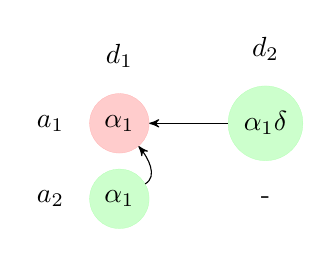
\begin{tikzpicture}[
    on_node/.style={circle, draw=red!30, fill=red!20, ultra thin, minimum size=4mm},
    opt_node/.style={circle, draw=green!30, fill=green!20, ultra thin, minimum size=4mm},
    null_node/.style={circle, draw=white!10, fill=white!10, ultra thin, minimum size=4mm},
    node distance=0.2cm,->,>=stealth',
    ]
    %Nodes
    \node (a1) {\(a_1\)};

    \node[on_node] (a1d1) [right=of a1] {$\alpha_1$};
    \node[opt_node] (a1d2) [right=1cm of a1d1] {\(\alpha_1\delta\)};

    \node[opt_node] (a3d1) [below=of a1d1] {$\alpha_1$}; 
    \node[null_node] (a3d2) [below=of a1d2] {-};

    \node (a3) [left=of a3d1] {\(a_2\)};

    \node (d1) [above=of a1d1] {\(d_1\)};
    \node (d2) [above=of a1d2] {\(d_2\)};

    % Edges
    \draw[->] (a1d2.west) -- (a1d1.east);
    \draw[->] (a3d1) to [out=30,in=310] (a1d1);
  \end{tikzpicture}}
  \caption[Tight Example]{A tight example with competitive ratio \(1 + \delta \). Online allocation indicated in red, Optimal allocation indicated in green and arrows indicate charging} 
  \label{fig:tight-model-1}
\end{figure}

The following example shows that the competitive ratio of Algorithm~\ref{alg:online-greedy-m1} is tight. Let the set of agents \(A=\{a_1, a_2\}\) and categories \(C=\{c_1, c_2\}\). Agent \(a_1\) is eligible under \(\{c_1,c_2\}\) and agent \(a_2\) is eligible only under \(\{c_2\}\).  The daily~supply: \(s_{1}=1 \text{ and } s_{2}=1\). The daily quota of each category on each day is set to \(1\). The  priority factor for both the agents  is~\(\alpha_1\). Assume that \(a_1\) is available on both the days whereas the agent \(a_2\) is available only on the first day.
Figure~\ref{fig:tight-model-1} depicts this example. 

\section{Online Algorithm for Model~$2$}\label{sec:onlineapprox}
We present an online algorithm which greedily maximizes utility on each day. We assume that the discounting factor of the agents is \(\delta\). Moreover each agent $a_k$ has a priority factor $\alpha_k$. Let $\alpha_{\max} = \max_i\{\alpha_i \mid \alpha_i \text{ is the priority factor of agent $a_i$}\}$ and $\alpha_{\min} = \min_i\{\alpha_i \mid \alpha_i \text{ is the priority factor of agent $a_i$}\}$. We show that this algorithm indeed achieves a competitive ratio of \(1+\delta + \frac{\alpha_{\max}}{\alpha_{\min}}\delta\). 

\emph{Outline of the Algorithm:} On each day \(d_i\), starting from day \(d_1\), we construct a bipartite graph \({H}_i=({A}_i\cup C, E_i, w_i)\) where set \({A}_i\) is the set of agents who are available on day \(d_i\) and are not vaccinated earlier than day $d_i$.  Let the weight of the
edge $(a_j , c_k) \in E_i$ be $w_i(a_j , c_k) = \alpha_j .\delta^{i-1}$. Let \(b'_{i,k}\) represent the capacity of \(c_k\in C\) in \(H_i\). In this graph, our algorithm finds a maximum weighted b-matching of size not more than the daily supply value \(s_i\). This can be found in polynomial time \cite{lawler2001combinatorial}. Lemma~\ref{lemma:max-size-max-wt} proves that the maximum weight b-matching is also a maximum cardinality b-matching of $H_i$.  

\begin{algorithm}
\caption{Online Algorithm for Vaccine Allocation}
\label{alg:online-greedy-m2}
\hspace*{\algorithmicindent} \textbf{Input:} An instance \(I\) of Model~2 \\
\hspace*{\algorithmicindent} \textbf{Output:} An allocation \(M:A\to(C\times D)\cup\{\varnothing\}\)

\begin{algorithmic}[1]
  \STATE Let \(D,A,C\) be the set of Days, Agents and Categories respectively.
  \STATE \(M(a_j)\gets \varnothing\) for each agent $a_j \in A$
  \STATE \(r_k \gets q_k\) for each category $c_k \in C$
  \FOR {day \(d_i\) in \(D\)}
  \STATE ${A}_i \gets \{ a_j \in A \mid a_j$ is available on $d_i$ and $a_j$ is not vaccinated\}
  \STATE $E_i=\{(a_j,c_k) \in {A}_i \times C \mid a_j$ is eligible to be vaccinated under category $c_k \}$
  \STATE Construct bipartite graph \({H}_i=({A}_i\cup C, E_i)\).
  \FOR {\(c_k\) in \(C\)}
  \STATE \(b'_{i,k} \gets min(q_{ik}, r_k)\) \COMMENT{Capacity for each \(c_k\) in \(H_i\)}
  \ENDFOR
    \STATE Find maximum weight b-matching \(N_i\)  in \(H_i\) of size at most \(s_i\).
  \FOR {each edge \((a_j,c_k)\) in \(M_i\)}
  \STATE \(M(a_j) \gets (c_k,d_i)\) \COMMENT{Mark \(a_j\) as vaccinated on day \(d_i\) under category \(c_k\)}
  \STATE \(r_k \gets r_k -1 \) \COMMENT {Update remaining overall quota}
  \ENDFOR
  \ENDFOR\\
  \RETURN \(M\)
\end{algorithmic}
\end{algorithm}

\subsection{Outline of the charging scheme}
We compare the solution obtained by Algorithm~\ref{alg:online-greedy-m2} with the optimal offline solution to get the worst-case competitive ratio for Algorithm~\ref{alg:online-greedy-m2}. Let $M$ be the output of Algorithm~\ref{alg:online-greedy-m2} and $N$ be an optimal offline solution. To compare $M$ and $N$, we devise a {\em charging scheme} similar to that in Section~\ref{sec:analysis-model-1}, by which each agent $a$ matched in $N$ {\em charges} a unique agent $a'$ matched in $M$. The amount charged, referred to as the {\em charging factor} here is the ratio of utilities obtained by matching $a$ and $a'$ in $M$ and $N$ respectively.

Properties of the charging scheme:
\begin{enumerate}
    \item Each agent matched in $N$ charges exactly one agent matched in $M$,
    \item Each agent matched in $M$ is charged by at most three agents matched in $N$, with charging factors at most $1,\delta$ and $\frac{\alpha_{\max}}{\alpha_{\min}}\delta$. This implies that the utility of $N$ is at most $(1+\delta+\frac{\alpha_{\max}}{\alpha_{\min}}\delta)$ times the utility of $M$.
\end{enumerate}

We divide the agents matched in $N$ into two types. Type $1$ agents are those which are matched in $M$ on an earlier day compared to that in $N$. Thus $a\in A$ is a Type $1$ agent if $a$ is matched on day $d_i$ in $M$ and on day $d_j$ in $N$, such that $i<j$. The remaining agents are called Type $2$ agents.
Our charging scheme is as follows:
    
\begin{enumerate}
    \item Type $1$ agents charge themselves with a charging factor $\delta$, since the utility associated with them in $N$ is at most $\delta$ times that in $M$. 
    
    \item Here onwards, we consider only Type $2$ agents and discuss the charging scheme associated with them.

Let $X_i$ be the set of Type $2$ agents matched on day $d_i$ in $N$, and let $Y_i$ be the set of agents matched on day $d_i$ in $M$. 

\begin{enumerate}
    \item {\em Case 1: $|X_i|\leq |Y_i|$: } From Lemma \ref{lemma:injection-exists} we claim that each agent $a_p \in X_i$ charges an agent in $a_q \in Y_i$ with $\alpha_p \leq \alpha_q$. Therefore the agents in $X_i$ charge the agents in $Y_i$ with a charging factor of $1$. 
    

\item {\em Case 2: $|X_i|=|Y_i|+z, z>0$: } Let $N_i$ and $M_i$ respectively be the restrictions of $N$ and $M$ to day $d_i$. We construct an auxiliary bipartite graph $G_i$ where $X_i\cup Y_i$ form one bipartition and categories form another bipartition. The edge set is $N_i\cup M_i$. For a category $c_k$, let $n_{j,k}$ and $m_{j,k}$ be the number of agents matched in $N$ and $M$ respectively, under category $c_k$ on day $d_j$. Then we set the quota of $c_k$ in $G_i$ to be $b_{i,k}=\min\{q_{i,k}, \max\{q_k-\sum_{j=1}^{i-1}n_{j,k}, q_k-\sum_{j=1}^{i-1} m_{j,k}\}\}$. This is the maximum of the quotas of $c_k$ that were available for computation of $N_i$ and $M_i$ respectively.
        
The charging scheme is given by the following. Consider the symmetric difference $M_i\oplus N_i$. Since $|N_i|=|M_i|+z$, there are exactly $z$ edge-disjoint alternating paths in $M_i\oplus N_i$ that start and end with an edge of $N$ \cite{NasreR17}. Let $\rho=\langle a_1,c_1,a_2,\ldots, a_k, c_k\rangle$ be one such path. Then $a_2,\ldots,a_{k-1}$ are matched in both $M_i$ and $N_i$, so they charge themselves with a charging factor of $1$. From Lemma \ref{lemma:injection-exists}, the agent $a_1$ charges $a_k$ with charging factor of at most $1$. It remains to decide whom $a_k$ charges.
        
Since $\rho$ terminates at $c_k$ with an $N_i$-edge, the number of agents matched to $c_k$ in $N_i$ is more than those matched to $c_k$ in $M_i$. In Lemma~\ref{lem:saturated}, we show that this can happen only because of exhaustion of $q_k$ in Algorithm~\ref{alg:online-greedy-m2} on or before day $d_i$. %since $|M_i|, |N_i|\leq s_i$ and $M_i$ is a maximum matching on day $d_i$. 
So agent $a_k$ can charge some agent $a_l$ matched to $c_k$ in $M$ on an earlier day, with charging factor $\frac{\alpha_{k}}{\alpha_{l}}\delta \leq \frac{\alpha_{\max}}{\alpha_{\min}}\delta$.
\end{enumerate}
\end{enumerate}

\begin{lemma}\label{lem:saturated}
If node $c_k$ is an end-point of a path $\rho$ in $G_i$, then $q_k$ is exhausted in Algorithm \ref{alg:online-greedy-m2} on or before day $d_i$. 
\end{lemma}
\begin{proof}
Suppose $c_k$ be an endpoint of $\rho$ in $G_i$. The number of agents matched to $c_k$ in $N_i$ is more than those matched to $c_k$ in $M_i$. We know that the daily supply $s_i$ of the day $d_i$ is an upperbound for both $|M_i|$ and $|N_i|$. Since $|N_i| = |M_i| + z$, we have $|M_i| < s_i$. From Algorithm \ref{alg:online-greedy-m2} we know that $M_i$ is a maximum-size b-matching in $H_i$ of size at most \(s_i\). If the capacity of $c_k$ is not saturated in $H_i$, then we can augment the path $\rho$ contradicting the maximality of $M_i$.  Since $c_k$ has more edges of $M_i$ than $N_i$ incident to it, from the definition of $b_{i,k}$, category $c_k$ must have exhausted the overall quota $q_k$ in Algorithm \ref{alg:online-greedy-m2} on or before day $d_i$. 
\end{proof}



%\begin{enumerate}
%    \item An agent who gets matched on day $d_i$ in the online solution and on day $d_j$ in the optimal solution, where $i<j$ charges itself. This forms the set $H_1$.
%    \item Along an augmenting path $\langle a_1,c_1,a_2,\ldots, a_k, c_k\rangle$ in $G_i$, $a_1,\ldots, a_{k-1}$ charge $a_2,\ldots,a_k$. Agent $a_k$ charges someone previously vaccinated in $ON$ in the same category $c_k$.
%    \item Note that $OPT_i$ matches more agents in $c_k$ than $ON_i$, and $|OPT_i|>|ON_i|$. So why did $ON_i$ not match more agents to $c_k$? The daily supply $s_i\geq %|OPT_i|>|ON_i|$. So $ON_i$ must have exhausted the overall %quota of $c_k$. Therefore, corresponding to $a_k$, there %must be an agent previously vaccinated by $ON$ in category %$c_k$. That agent is charged for $a_k$ with charging factor %$\delta$.
%\end{enumerate}

% \subsection{Analysis of the Algorithm}\label{sec:analysis-model-generic}
% To show that Algorithm~\ref{alg:online-greedy} achieves the desired competitive ratio, we introduce a \emph{charging scheme} - a mapping technique to compare the computed allocation with an optimal allocation. We say that an agent \(a\) who is vaccinated by an optimal allocation \emph{charges} an agent \(b\) with a \emph{charging factor}. To be precise, we show that the set \(S_{OPT}\) of agents who are vaccinated by an optimal allocation can be partitioned into three parts \(H_1, H_2 \text{ and } H_3\) such that any agent \(b\) who is vaccinated by the online allocation (computed by Algorithm~\ref{alg:online-greedy}) is charged by at most one agent from each part. Furthermore, each agent in \(H_1\cup H_3\) charges $b$ with a charging factor of \(\delta\), and each agent in \(H_2\) charges at most one agent with a charging factor \(1\).

% Let \(ON\) be an allocation computed by Algorithm~\ref{alg:online-greedy} on an instance \(I\), and let \(OPT\) be an optimal allocation on the same instance \(I\). Recall that an allocation \(M\) is of the form \(M:A\to(C\times D)\cup\{\varnothing\}\). Let \(S_{OPT}\) and \(S_{ON}\) be the sets of agents who got vaccinated by \(OPT\) and \(ON\) respectively. Now, \(H_1 \subseteq S_{OPT} \) can be described as the set of agents who are vaccinated by \(ON\) at least one day before they are vaccinated by \(OPT\) That is,

% \begin{align*}
%   H_1&=\{a\in S_{OPT} \mid OPT(a)=(c_i,d_j),\  ON(a)=(c_k,d_\ell), d_\ell<d_j\}
% \end{align*}

% For every agent \(a\in H_1\), \(a\) charges itself i.e. \(a \in S_{ON}\). Therefore, by definition, no two agents in \(H_1\) charge the same agent, and every agent in \(H_1\) charges exactly one agent in \(S_{ON}\). Since the utility associated with vaccinating $a$ in \(OPT\)is at most $\delta$ times that in \(ON\),the charging factor is $\delta$ in this case.

% Let \(S'_{OPT} = S_{OPT}\setminus H_1\). %be the remaining agents from \(S_{OPT}\) who are not in \(H_1\).

% To construct the parts \(H_2\) and \(H_3\), we first partition the agents in \(S'_{OPT}\) based on the day on which they got vaccinated by \(OPT\). That is, \[ S' = X_1\uplus X_2 \uplus \cdots \uplus X_{r=|D|} \]where,
% \begin{align*}
%   X_i &= \{a\in S' \mid a \text{ is vaccinated on day } d_i \text{ by } OPT  \} &&\forall {i\in\{1,2,\cdots,|D|\}}\\
% \end{align*}
% Similarly, let\[ S'_{ON} = Y_1\uplus Y_2 \uplus \cdots \uplus Y_{r=|D|} \] where,
% \begin{align*}
%   Y_i &= \{a\in S'_{ON} \mid a \text{ is vaccinated on day } d_i \text{ by } ON  \} &&\forall {i\in\{1,2,\cdots,|D|\}}\\
% \end{align*}

% Now, to construct the sets \(H_2\) and \(H_3\), we go over each set \(X_i\) and decide whether to include either the whole set \(X_i\) or a subset of it into \(H_2\). For each set \(X_i\), if \(|X_i|\le|Y_i|\), then we add \(X_i\) to \(H_2\).  This means the agents in \(X_i\) charge the agents in \(Y_i\), and the charging factor is \(1\) as the utility associated with vaccinating an agent in $X_i$ and its counterpart in $Y_i$ is the same. Since  \(|X_i|\le|Y_i|\), we can choose any injective mapping from \(X_i\) to \(Y_i\) for this charging scheme. On the other hand, if \(|X_i|=|Y_i|+m,\ m>0\), then we carefully pick \(m\) agents from \(X_i\) and put them in \(H_3\) and the remaining agents to \(H_2\). In the following sections, we describe how to pick these agents and how these agents charge agents in \(S_{ON}\).

% \begin{algorithm}
% \caption{Algorithm to construct \(H_2\) and \(H_3\)}
% \label{alg:partition-h2-h3}
% \begin{algorithmic}[1]
%   \State Initialize \(H_2,H_3 \gets \varnothing\)
%   \For {\(i = 1, 2, \ldots, r=|D|\)}
%   \If{\(|X_i| \le |Y_i|\)}
%   \State \(H_2 \gets H_2 \cup X_i\)
%   \ElsIf{\(|X_i| = |Y_i| + m, m>0\)}
%   \State \(( \mathcal{U}_{d_i}, \mathcal{V}_{d_i}) \gets\textsc{Careful-partition}(X_i)\)
%   \State \(H_2\gets H_2 \cup  \mathcal{U}_{d_i}\)
%   \State \(H_3 \gets H_3 \cup  \mathcal{V}_{d_i}\) \Comment{\(| \mathcal{V}_{d_i}|=m\)}
%   \EndIf
%   \EndFor
%   \Procedure{Careful-partition}{$X_i$}
%   \State Let  \(A_i \gets \{a\in A \mid a \text{ is available on day } d_i, ON(a)=(c_k,d_j)\ s.t\  d_j\ge d_i\}\)
%   \State Let \(M_i^{ON} \gets \{(a_j,c_k) \mid a_j\in A_i \text{ is vaccinated on day } d_i \text{ under } c_k \text{ by } ON\}\)
%   \State Let \(M_i^{OPT} \gets \{(a_j,c_k) \mid a_j\in A_i \text{ is vaccinated on day } d_i \text{ under } c_k \text{ by } OPT\}\)
%   \State \(M \gets M_i^{ON} \triangle M_i^{OPT}\) \Comment{Symmetric difference}
%   \State Compute \(P_i\) the set of \(m\) edge disjoint \(M_i^{ON}\)-augmenting paths in \(M\).
%   \State \( \mathcal{V}_{d_i} \gets \{a \in A_i \mid \text{\(a\) is a penultimate agent in one of the paths in \(P_i\)} \}\)
%   \State \( \mathcal{U}_{d_i} \gets X_i\setminus  \mathcal{V}_{d_i}\)\\
%   \Return \(( \mathcal{U}_{d_i}, \mathcal{V}_{d_i})\)
%   \EndProcedure
% \end{algorithmic}
% \end{algorithm}


% Consider the case when \(|X_i| = |Y_i|+m\) such that \(m>0\) for some \(i\). Now, to partition \(X_i\) as \(X_i = \mathcal{U}_{d_i}\uplus  \mathcal{V}_{d_i}\), we construct an auxiliary bipartite graph \(G_i = (A_i\cup C, E_i)\), where \(A_i\) is the set of agents, who are available on day \(d_i\) and are not vaccinated until day \(d_{i-1}\) by \(ON\) i.e. 
% $A_i = \{a\in A \mid \ a \text{ is available on day } d_i \text{ and } ON(a)\ne(c_k,d_j)\ \forall  d_j< d_i \}$.


% There is an edge \((a_i,c_k)\) if \(a_i\) is eligible under category \(c_k\). To view allocations as \emph{b-matchings}, we introduce capacity functions \(b_{ON}^i:C\to \mathbb{Z}_{\ge 0}\) and \(b_{OPT}^i:C\to \mathbb{Z}_{\ge 0}\), which is the minimum of daily quota \(q_{ik}\) and total \emph{remaining} quota from the overall quota \(q_k\). Let \(n_{(i,k)}^{ON}\) and \(n_{(i,k)}^{OPT}\) represent total number of agents who got vaccinated under category \(c_k\) on or before day \(d_i\) by \(ON\) and \(OPT\) respectively. Then,
% \begin{align*}
%   b^{ON}_i(c_k) &= \min(q_{ik}, q_k-n_{(i-1,k)}^{ON})\\
%   b^{OPT}_i(c_k) &= \min(q_{ik}, q_k-n_{(i-1,k)}^{OPT})\\
% \end{align*}

% %b^i(c_k) &= max( b_{ON}^i(c_k),  b_{OPT}^i(c_k))
% Now, it is apparent that an allocation by \(ON\) for \(A_i\) on day \(d_i\) is a valid matching in \((G_i,b^{ON}_i)\). Similarly, an allocation by \(OPT\) can be viewed as a matching in \((G_i,b^{OPT}_i)\). Let us call these matchings as \(M_i^{ON}\) and \(M_i^{OPT}\) respectively.
% \begin{align*}
%   M_i^{ON} &= \{(a_j,c_k) \mid a_j\in A_i \text{ is vaccinated on day } d_i \text{ under } c_k \text{ by } ON\}\\
%   M_i^{OPT} &= \{(a_j,c_k) \mid a_j\in A_i \text{ is vaccinated on day } d_i \text{ under } c_k \text{ by } OPT\}\\
% \end{align*}

% It is clear that \(|M_i^{OPT}| = |X_i|\) and \(|M_i^{ON}| = |Y_i|\). %The set \(X_i\) is a set of agents whereas \(M_i^{OPT}\) is a set of edges - one edge per each agent in \(X_i\).\\

% Let \(b_i:C \to \mathbb{Z}_{\ge 0}\) be defined as
% \begin{align*}
%   b_i(c_k) &= \max(b^{ON}_i(c_k), b^{OPT}_i(c_k))
% \end{align*}

% Clearly, both \(M_i^{OPT}\) and \(M_i^{ON}\) are valid b-matchings in \((G_i,b_i)\). We use the following lemma to get \(m\) edge disjoint \(M_i^{ON}\)-augmenting paths \(P_i\) in \((G_i,b_i)\).
% \begin{lemma}
%   If \(|M_i^{OPT}| - |M_i^{ON}| = m > 0\), then there exists \(m\) edge disjoint \(M_i^{ON}\)-augmenting paths in \((G_i,b_i)\).
% \end{lemma}
% \begin{proof}
%   We prove this by principle of mathematical induction.
%   We are given that \(|M_i^{OPT}| - |M_i^{ON}| = m > 0\).
%   \paragraph{Base Case:} Let \(m=1\)
%   As \(|M_i^{OPT}| > |M_i^{ON}|\), there exists an \(M_i^{ON}\)-augmenting path in \((G_i,b_i)\) whose unmatched edges are from \(M_i^{OPT}\).
%   \paragraph{Induction Hypothesis: } Suppose the claim hold for \(m=k\) for some \(k\). That is, there exists \(k\) edge disjoint  \(M_i^{ON}\)-augmenting paths in \((G_i,b_i)\).

%   Now, let \(|M_i^{OPT}|-|M_i^{ON}|= k+1\). Since, \(|M_i^{OPT}|>|M_i^{ON}|\), there exists at least one  \(M_i^{ON}\)-augmenting path \(p\) in \((G_i,b_i)\) whose unmatched edges are from \(M_i^{OPT}\). Since \(p\) contains one more edge from \(M_i^{OPT}\) than \(M_i^{ON}\), \(|M_i^{OPT}\setminus~p|-|M_i^{ON}\setminus~p|=k>0\). By induction hypothesis, there exists \(k\) edge disjoint \(M_i^{ON}\)-augmenting paths in \((G_i,b_i)\). These \(k\) paths along with \(p\), give \(k+1\) many edge disjoint \(M_i^{ON}\)-augmenting paths in \((G_i,b_i)\).
% \end{proof}

% Let \(C_i\) be the set of categories which are end points of paths in \(P_i\). We consider the set \( \mathcal{V}_{d_i}\) of agents who are penultimate vertices of these paths. The sets can be formally defined as:  

% \begin{align*}
%              C_i = \{c_k \in C \mid\  &c_k \text{ is an end point of a path } p \in P_i\}\\
%    \mathcal{V}_{d_i} = \{a \in A_i \mid\  &(a,c_k) \in G_i \text{ for some } c_k\in C_i,\\
%                                     &a \text{ is a penultimate vertex of the paths in } P_i\}
% \end{align*}

% Let \(\mathcal{V}\) be the union of \(\mathcal{V}_{d_i}\) over all days.
% \begin{align*}
%   \mathcal{V} \defeq \bigcup_{d_i \in D} \mathcal{V}_{d_i}
% \end{align*}

% We repartition \(\mathcal{V}\) in terms of categories as follows
% \begin{align*}
%   \mathcal{V} &= \mathcal{V}_{c_1} \uplus \mathcal{V}_{c_2} \uplus \cdots \uplus \mathcal{V}_{c_k} &&\text{where,}\\
%   \mathcal{V}_{c_j} &= \{a\in \mathcal{V} \mid a \text{ is vaccinated under category } c_j \text{ by } OPT\}\\
% \end{align*}

% To show that \(\mathcal{V}_{d_i} \uplus \mathcal{U}_{d_i} = X_i\), \marginpar{\textcolor{red}{Is $\mathcal{U}_{d_i}$ defined at this stage?}} we first show that \(\mathcal{V}_{d_i} \subseteq X_i\).  
% \begin{lemma}
%   \( \mathcal{V}_{d_i}\subseteq X_i\)
% \end{lemma}
% \begin{proof}
%   For any agent \(a\in \mathcal{V}_{d_i}\), consider the \(M_i^{ON}\)-augmenting path \(p\) which has \((a,c_k)\) as one of its end edges. Since \(p\) is a  \(M_i^{ON}\)-augmenting path, \((a,c_k)\in M_i^{OPT}\). Thus \(a\) is vaccinated by \(OPT\) on day \(d_i\).

%   As \(a\in A_i\), \(a\) is not vaccinated by \(ON\) on or before day \(d_{i-1}\). And \(a\) got vaccinated by \(OPT\). Therefore, \(a \notin H_1\).  Which implies \(a\in S'\).

%   Hence, \(a\in X_i\).
% \end{proof}


% \begin{remark}\label{remark:m-agents}
%   If \(|P_i|=m\), then \(|\mathcal{V}_{d_i}|=m\).
% \end{remark}
% Remark~\ref{remark:m-agents} holds as the paths in \(P_i\) are edge disjoint, and \(\mathcal{V}_{d_i}\) is the set of penultimate vertices of these paths.

% Let \( \mathcal{U}_{d_i}=X_i\setminus  \mathcal{V}_{d_i}\). Now, while constructing \(H_2\) and \(H_3\), we add \( \mathcal{U}_{d_i}\) to \(H_2\) and \( \mathcal{V}_{d_i}\) to \(H_3\). Since \(|Y_i| = | \mathcal{U}_{d_i}|\), and by the construction of \(H_2\), the agents in \(Y_i\) are not yet charged by anyone from \(H_2\), the agents in \( \mathcal{U}_{d_i}\) charge the agents in \(Y_i\) with a charging factor of \(1\). Any arbitrary injective mapping works for this charging scheme.

% All that is left to prove now, is that each agent \(a\) in \(H_3\) who got vaccinated by \(OPT\) on some day \(d_j\), can uniquely charge an agent who got vaccinated by \(ON\) on some day \(d_k<d_j\). We prove this with the help of following lemmas.



% For all \(c_k \in C_i\), the set \( \mathcal{V}_{c_k} \cap \mathcal{V}_{d_i} \subseteq \mathcal{V}\) is the set of agents from \(\mathcal{V}\) who are penultimate vertices of paths in \(P_i\) ending at category \(c_k\).  These agents are vaccinated by \(OPT\) on day \(d_i\) under category \(c_k\). Suppose \(| \mathcal{V}_{c_k} \cap \mathcal{V}_{d_i}| =l\), then we have the following lemma.

% \begin{lemma}
%   \label{lemma:end-point}
%   If \(c_k\in C_i\) is the end point of \(l\) many paths from \(P_i\), then\\
%   \(b^i_{OPT}(c_k)~\ge~b^i_{ON}(c_k)~+~l\).
% \end{lemma}
% \begin{proof}
% We know that \(|M_i^{OPT}| = |M_i^{ON}| + l \le s_i\). Therefore the size of \(M_i^{ON}\) is strictly less than the daily supply \(s_i\), i.e,  \(|M_i^{ON}| < s_i\). Furthermore, the matching \(M_i^{ON}\) is a maximum size b-matching on \((G_i,b^i_{ON})\). If the capacity of \(c_k\) is not saturated in \((G_i,b^{ON}_i)\), then there exists an augmenting path \(p\in P_i\). This contradicts the maximality of \(M_i^{ON}\) as \(|M_i^{ON} \triangle\ p|>|M_i^{ON}|\). Therefore, the number of agents vaccinated on day \(d_i\) under category \(c_k\) is equal to \(b^i_{ON}(c_k)\).

%   From our assumption, there are \(l\) many \(M_i^{ON}\)-augmenting paths ending at \(c_k\) in \((G_i,b_i)\). From Remark~\ref{remark:m-agents}, we know that each augmenting path has a unique \(M_i^{OPT}\) edge to \(c_k\). If we apply every \(M_i^{ON}\)-augmenting path from \(P_i\), then the number of \(M_i^{ON}\) edges incident to \(c_k\) increases by \(l\). As \(M_i^{ON}\) saturates \(c_k\) in \((G_i,b_i^{ON})\), the capacity \(b_i(c_k) \ge b_i^{ON}(c_k) + l\). From the fact that \(b_i(c_k) = \max(b_i^{OPT}(c_k), b_i^{ON}(c_k))\), we can conclude that \(b_i(c_k) = b_i^{OPT}(c_k)\). Thus, \(b^i_{OPT}(c_k)~\ge~b^i_{ON}(c_k)~+~l\).
% \end{proof}

% \begin{corollary}\label{corollary:strict-less}
%   For each \(c_k \in C_i\), the online capacity \(b^i_{ON}(c_k) = q_k-n_{(i-1,k)}^{ON}\)
% \end{corollary}
% \begin{proof}
%   By definition  \(b_{ON}^i(c_k) = min(q_{ik}, q_k-n_{(i-1,k)}^{ON})\), From the above lemma, we know \(b^i_{OPT}(c_k)>b^i_{ON}(c_k)\). Moreover, \(q_{ik} \ge b^i_{OPT}\). Therefore, \(q_{ik}>b^i_{ON}\). Hence, \(b^i_{ON}(c_k) = q_k-n_{(i-1,k)}^{ON}\).
% \end{proof}

% % {\color{red}Now, using Corollary~\ref{corollary:strict-less} and Lemma~\ref{lemma:end-point}, the following theorem shows that every agent in \( \mathcal{V}_k\), for all \(c_k\in C_i\), can uniquely charge some agent who got vaccinated by \(ON\) under category \(c_k\) at least one day earlier. }

% \begin{corollary}\label{corollary:category-saturation}
%   For each \(c_k \in C_i\), the total number of agents vaccinated until (including) day \(d_i\) is \(q_k\)
% \end{corollary}
% \begin{proof}
%   % Without loss of generality, assume \(i<j\). From Corollary~\ref{corollary:strict-less}, we know that the capacity of category \(c_k\) on day \(d_i\) is \(b^i_{ON}  = q_k-n_{(i-1,k)}^{ON}\). As \(M_{i}^{ON}\) is a maximum size b-matching of size at most \(s_i\), and as \(|M_{i}^{OPT}|\le s_i\), It is clear that number of agents vaccinated by \(ON\) on day \(d_i\) under category \(c_k\)is exactly equal to it's capacity \(c_k\). Because otherwise, the size of \(M_i^{ON}\) can be increased by augmenting along one of the \(M_{i}^{ON}\)-augmenting path ending at \(c_k\). Therefore the total number of agents vaccinated by \(ON\) under category \(c_k\) on or before day \(d_i\) is
% We know that the number of agents vaccinated until day \(d_{i-1}\) under category \(c_k\) is \(n^{ON}_{(i-1,k)} \). From Corollary~\ref{corollary:strict-less} the number of agents vaccinated under category \(c_k\) on day \(d_i\) is \(q_k-n_{(i-1,k)}^{ON}\). Therefore, the total number of agents vaccinated under category \(c_k\) until day \(d_i\) is:
%   \begin{align*}
%     &= n^{ON}_{(i-1,k)} + q_k-n_{(i-1,k)}^{ON}\\
%     &= q_k\\
%   \end{align*}
% \end{proof}

% From Corollary~\ref{corollary:category-saturation}, we learn that the overall~quota \(q_k\) of the category is saturated by day \(d_i\).

% Now, we compare the number of agents vaccinated by \(OPT\) and \(ON\) until day \(d_{i-1}\) under category \(c_k\).


% \begin{lemma}\label{lemma:end-point-2}
%   If \(c_k \in C_i\) is the end point of \(l\) many paths from \(P_i\), then \( n_{(i-1,k)}^{OPT} \le n_{(i-1,k)}^{ON} - l\).   
% \end{lemma}
% \begin{proof}
%   From Corollary~\ref{corollary:strict-less}, Capacity \(b^i_{ON}(c_k) = q_k-n_{(i-1,k)}^{ON}\). From Lemma~\ref{lemma:end-point}, we know that  \(b^i_{OPT}(c_k)~\ge~b^i_{ON}(c_k)~+~l\). Therefore,
%   \begin{align*}
%     b^i_{OPT}(c_k)~\ge~ q_k-n_{(i-1,k)}^{ON}~+~l
%   \end{align*}
%   We know that \ \  \(b^i_{OPT}(c_k) = min(q_{ik}, q_k-n_{(i-1,k)}^{OPT}) \). Therefore,
%   \begin{align*}
%     &q_k-n_{(i-1,k)}^{OPT} \ge q_k-n_{(i-1,k)}^{ON} + l\\[10pt]
%       \implies& n_{(i-1,k)}^{OPT} \le n_{(i-1,k)}^{ON} - l
%   \end{align*}
%   % That is, the number of agents who got vaccinated by \(ON\) until day \(d_{i-1}\) under category \(c_k\) is at least \(l\) more than the number of agents who got vaccinated by \(OPT\) until day \(d_{i-1}\) under category \(c_k\). Therefore, there are sufficient number of agents for these \(l\) agents to charge to. Thus, the \(l\) penultimate agents of category \(c_k\) uniquely charge some \(l\) agents who were vaccinated by \(ON\) on or before day \(d_{i-1}\) under category \(c_k\) with a charging factor of \(\delta\).  
% \end{proof}


% \begin{theorem}\label{thm:main}
%   Every agent \(a \in \mathcal{V}_{c_k} \cap \mathcal{V}_{d_i}\) can uniquely charge an agent who is vaccinated by \(ON\) under the same category \(c_k\) on some day \(d_j\), where \(d_j < d_i\).
% \end{theorem}
% \begin{proof}
%   If \(\mathcal{V}_{c_k} = \varnothing\), then the theorem vacuously holds. Suppose \(\mathcal{V}_{c_k} \neq \varnothing\). Then by Corollary~\ref{corollary:category-saturation}, The overall quota of category \(c_k\) is saturated by \(ON\) for the first time on some day \(d_q\).

%   Now, we claim that \(\mathcal{V}_{c_k}\) does not contain any agent who is vaccinated on or before day \(d_{q-1}\). Because, if \(a \in \mathcal{V}_{c_k} \cap \mathcal{V}_{d_p}\) with \(d_p < d_q \), then from Corollary~\ref{corollary:category-saturation}, the overall quota of \(c_k\) is saturated by \(ON\) on day \(d_p\), which is a contradiction as we assumed \(d_q\) to be the first such day.

%   Suppose \(|\mathcal{V}_{c_k} \cap \mathcal{V}_{d_q}| = l\), then from Lemma \ref{lemma:end-point-2}, the number of agents who got vaccinated by \(ON\) until day \(d_{q-1}\) under category \(c_k\) is at least \(l\) more than the number of agents who got vaccinated by \(OPT\) until day \(d_{q-1}\) under category \(c_k\). Therefore the agents in \(|\mathcal{V}_{c_k} \cap \mathcal{V}_{d_q} |\) can uniquely charge \(l\) agents  who are vaccinated by \(ON\) on or before day \(q-1\).
  
%   Clearly \(|\mathcal{V}_{c_k}| \leq q_k \). Also, the number of agents vaccinated until day \(d_q\) by \(ON\) under category \(c_k\) is \(q_k\). Therefore the agents in \(\mathcal{V}_{c_k}\) who are vaccinated after day \(d_q\) can also uniquely charge some agent who got vaccinated by on \(ON\) under category \(c_k\) on or before day \(d_q\).

%   Therefore, every agent \(a \in \mathcal{V}_{c_k} \cap \mathcal{V}_{d_i}\) can uniquely charge an agent who is vaccinated by \(ON\) under the same category \(c_k\) on some day \(d_j\) before \(d_i\).
% \end{proof}

% It is clear that \(\bigcup_{d_i \in D}\mathcal{V}_{d_i} = \mathcal{V} = \bigcup_{c_k \in C}\mathcal{V}_{c_k}\) and \(\mathcal{V} = H_3\). As Theorem~\ref{thm:main} holds for every \(\mathcal{V}_{c_k}\), every agent in \(H_3\) can uniquely charge some agent with a charging factor of \(\delta\)

% \begin{proof}[of Theorem~\ref{thm:gen-on-same-utility}~(ii)]
%   Let $a_q$ be an agent who is vaccinated by the online matching \(M\) on day $i$. Then $a_q$ can be charged by at most three agents matched in \(N\). Suppose $a_q$ is vaccinated by the optimal matching \(N\) on some day $i' >i$. Assume that the agent $a_p$ and  of type 2 who also charges $a_p$. If the discounting factor of $a_q$ and $a_p$ are $\delta_q$ and $\delta_p$ respectively, then    
%   \begin{align*}
%     \frac{\delta_p^i + \delta_q^{i'}}{\delta_q^i}\  =\  \left(\frac{\delta_p}{\delta_q}\right)^i + {\delta_q^{i'-i}} \  \leq\  1 + \delta_q 
%   \end{align*}
% The last inequality follows as \(\delta_p \leq \delta_q \text{ and }i' > i\).  Therefore the utility obtained by $a_p$ and $a_q$ in $M_i$ is atmost $1 + \delta_q$ times the the utility of $a_q$ in $M_i$. Therefore the competitive ratio of Algorithm~\ref{alg:online-greedy-m1} is at most $1 + \max_i\{1 + \delta_i\}$.  
% \end{proof}


\subsection {Tight Example}
The following example shows that the competitive ratio of Algorithm~\ref{alg:online-greedy-m2} is tight. Let set of agents \(A=\{a_1, a_2, a_3\}\) and categories \(C=\{c_1, c_2\}\). Agent \(a_1\) is eligible under \(\{c_1,c_2\}\). Agent \(a_2\) is eligible only under \(\{c_1\}\) and agent \(a_3\) is eligible only under \(\{c_2\}\).  The daily~supply: \(s_{1}=1 \text{ and } s_{2}=2\). Overall~quotas: \(q_1=1 \text{ and } q_2=2\). The daily quota of each category on each day is set to \(1\). The utility discounting factor for each agent is~\(\delta\).  The priority factor of the agent $a_i$ is $\alpha_i$ for $i = 1,2,3$. We assume that $0 \leq \alpha_1 = \alpha_3 < \alpha_2 \leq 1$. Agent \(a_1\) is available on both the days.  Agent \(a_3\) is available only on the first day, whereas agent $a_2$ is available only on the second day.  
Figure~\ref{fig:tight-general} depicts this example. 
\begin{figure}
  \centering
  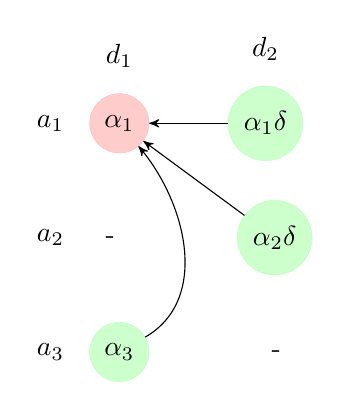
\begin{tikzpicture}[
    on_node/.style={circle, draw=red!30, fill=red!20, ultra thin, minimum size=4mm},
    opt_node/.style={circle, draw=green!30, fill=green!20, ultra thin, minimum size=4mm},
    null_node/.style={circle, draw=white!10, fill=white!10, ultra thin, minimum size=4mm},
    node distance=0.2cm,->,>=stealth',
    ]
    %Nodes
    \node (a1) {\(a_1\)};
    \node (a2) [below=1cm of a1] {\(a_2\)};
    \node (a3) [below=1cm of a2] {\(a_3\)};

    \node[on_node] (a1d1) [right=of a1] {$\alpha_1$};
    \node[opt_node] (a1d2) [right=1cm of a1d1] {\(\alpha_1\delta\)};
    
    \node[null_node] (a2d1) [right=of a2] {-};
    \node[opt_node] (a2d2) [right=1.35cm of a2d1] {\(\alpha_2\delta\)};
    
    \node[opt_node] (a3d1) [right= of a3] {$\alpha_3$}; 
    \node[null_node] (a3d2) [right=1.35cm of a3d1] {-};

    

    \node (d1) [above=of a1d1] {\(d_1\)};
    \node (d2) [above=of a1d2] {\(d_2\)};

    % Edges
    \draw[->] (a1d2.west) -- (a1d1.east);
    \draw[->] (a2d2) -- (a1d1);
    \draw[->] (a3d1) to [out=30,in=310] (a1d1);
  \end{tikzpicture}
  \caption[Tight Example]{A tight example with competitive ratio \(1+\delta+\frac{\alpha_2}{\alpha_1}\delta\). Online allocation indicated in red, Optimal allocation indicated in green and arrows indicate charging} 
  \label{fig:tight-general}
\end{figure}

Since the daily supply of day \(d_1\) is \(1\), vaccinating \(a_1\) maximizes the utility gained on the first day. Hence there exists a run of Algorithm~\ref{alg:online-greedy-m2} where \(a_1\) is  vaccinated under category \(c_1\) on day \(d_1\). In this run, agent \(a_2\) cannot be vaccinated on day \(d_2\) as she is eligible only under category \(c_1\) and overall quota of category \(c_1\) is exhausted. Hence, total utility gained by the online allocation is \(\alpha_1\). Whereas in a optimal allocation scheme all the agents can be vaccinated. Vaccinate agent \(a_3\) on day \(d_1\) under category \(c_2\), agent \(a_1\) and \(a_2\) on day \(d_2\) under categories \(c_2,c_1\) respectively. This sums to a total utility of \(\alpha_3+\alpha_1\delta+{\alpha_2}\delta\). Therefore the competitive ratio of the online algorithm is $\frac{\alpha_3+\alpha_1\delta+{\alpha_2}\delta}{\alpha_1} = \frac{\alpha_1+\alpha_1\delta+{\alpha_2}\delta}{\alpha_1} = 1+\delta+\frac{\alpha_{\max}}{\alpha_{\min}}\delta$. The first equality holds as $\alpha_1 = \alpha_3$. The second equality holds as $\alpha_{\max} = \alpha_2$ and $\alpha_{\min} = \alpha_1$.


 \section{Strategy-proofness of the online algorithm}
We give the details of the Pure Nash Equilibrium here.
% 1. Offline optimal algorithm is prone to strategic manipulation where agents can benefit by hiding availability. 
% 2. There is a pure Nash equilibrium in the offline setting such that the utility of the Nash equilibrium has the same value as that of the online algorithm. 
% 3. If there are multiple pure Nash equilibria, it is not clear which one will people land up into. To avoid landing up into bad Nash equilibrium, the online algorithm is useful.
% 4. The online algorithm gives a $1+\delta$-approximation to optimal solution, hence the online solution is a $1+ \delta$-approximation to any Nash equilibrium.

% -----------------------


%minimize the number of days she reports as available while still being able to receive the resource. This corresponds to the reluctance of the agent to lose out on outside options that the agent could have exercised by not turning up to wait in line for the vaccine.
%Agents can be strategic by under-reporting the categories from which they qualify for the resource. Further, agents also have the option of marking only a subset of their actual available days as available.
\subsection{Pure Nash equilibrium}\label{sec:Nash-eq}
The offline algorithm might choose any arbitrary matching that maximizes the utility. We present a deterministic tie-breaking rule similar to the one used in \cite{Aziz21} to force the algorithm to pick a unique matching. For this, we fix an ordering \(\pi\) on agents. We show the existence of a pure Nash equilibrium under the deterministic tie-breaking. We cast our problem as a linear program as given in Fig~\ref{fig:lp1}.

\begin{figure}
\begin{alignat*}{2}
  & \text{maximize: } & & \smashoperator[l]{\sum_{\substack{i\in A, j\in C,\\ k\in D}}} u_{ik}.x_{ijk} \\
    & \text{subject to: }& \quad & \smashoperator[l]{\sum_{i\in A,j\in C}}
                    \begin{aligned}[t]
                        x_{ijk} & \le s_k,& \forall k & \in D\\[3ex]
                    \end{aligned}\\
    &             & \quad & \smashoperator[l]{\sum_{i\in A\ \ \ \ }}
                    \begin{aligned}[t]
                        x_{ijk} & \le q_{jk},& \forall (j,k) & \in C\times D\\[3ex]
                    \end{aligned}\\
    &             & \quad & \smashoperator[l]{\sum_{j\in C,k\in D}}
                    \begin{aligned}[t]
                        x_{ijk} & \in [0,1],& \forall i & \in A\\[3ex]
                    \end{aligned}\\
    &             & \quad & \quad\ \ \ \ \ \ \ \
                    \begin{aligned}[t]
                        x_{ijk} & \in [0,1],& \forall (i,j,k) & \in A\times C \times D\\[3ex]
                    \end{aligned}\\
\end{alignat*}
\caption{Here $u_{ik}$ is the utility value of agent $i$ on day $k$, and $ s_k \& q_{jk}$ are the daily supply and daily quotas respectively.}
\label{fig:lp1}
\end{figure}

 It can be seen that this LP models the network flow formulation of our problem stated in Section~\ref{sec:offline-optimal-algorithm}. It is known (\cite{lawler2001combinatorial}) that the polytope arising from the network flow problem is integral. To impose the deterministic tie breaking, we modify the objective function as follows. 
 
 \begin{align*}
  \text{maximize\ }& \smashoperator[l]{\sum_{\substack{i\in A, j\in C,\\ k\in D}}} u_{ik}.x_{ijk} + \lambda \times REG, \text{where}\\
  REG &= \sum_{i \in A} \frac{\sum_{k \in D, j \in C} x_{ijk}}{2^{\pi(i)}}
\end{align*}

For a sufficiently small \(\lambda\) \((\lambda < \delta^{|D|+1})\), the difference between utilities of any two allocations is greater than \(REG\). Therefore, the linear program in Figure~\ref{fig:lp1} maximizes the objective function in Fig~\ref{fig:lp1}, but breaks ties to maximize \(REG\).

Let \(A_{d_i}\) be defined as the set of agents matched on a day \(d_i\in D\) and \(A_\infty\) be the set of unmatched agents at the end of a run of the Algorithm~\ref{alg:online-greedy-m1}. Let agent \(a_p\) be matched on \(d_i\) (WLOG, assume all unmatched agents are matched on day \(\infty\). Now, we present a proof of Theorem~\ref{thm:nash}. 

\begin{proof}(of Theorem~\ref{thm:nash})
%In the profile described above, agent \(a_p\) is matched on \(d_i\).
Suppose the agent \(a_p\) is matched on day $d_i$, and deviates to reporting a subset of the actual available days. %Let \({D_{p_i}} \subseteq D_p\) be the days prior to \(d_i\).

If agent \(a_p\) gets matched on a day \(d_j\), $j<i$, because of misreporting her available days, then some agent \(a_q\) on day \(d_j\) will remain unmatched. This follows, since on any given day, the matching  computed by algorithm \ref{alg:online-greedy-m1} is of maximum size and all agents other than \(a_p\) turn up on at most one day. The rest of the matching will remain unchanged.
But, agent \(a_q\) is prioritized by \(\pi\) over agent \(a_p\). Otherwise, algorithm \ref{alg:online-greedy-m1} would have matched \(a_p\) and not \(a_q\) on day \(d_j\). Hence, agent \(a_p\) cannot replace agent \(a_q\) on day \(d_j\) even after misreporting her availability.

Therefore agent \(a_p\) has no advantage in deviating from the strategy. Hence, the above matching is a pure Nash equilibrium.
\end{proof}

% It is reasonable to believe agents are not computationally strong entities with good beliefs about the availability of other agents. Hence, coordinating on a pure Nash equilibrium that maximizes utility will be hard. Agents might play an equilibrium with a worse performance. But, they will not be able to play an equilibrium that is substantially better than the one described above (the utility of the above described equilibrium is exactly equal to the utility of the \(1+\delta\)--approximation algorithm \ref{alg:online-greedy-m1}).

% The online approximation reduces the scope for strategic behavior from agents. Agents, at any point must decide on signing up availability one day at a time. But, deciding this requires far less information than the one needed to decide its strategy while participating in the offline optimal.
% Thus, it might be desirable to run the online algorithm with strategic agents, despite the offline optimal possibly returning a better utility.
\section{Experimental Evaluation}\label{sec:simulation}
In Section~\ref{sec:model1} we prove worst-case guarantees for the online algorithm. We also give a tight example instance achieving a competitive ratio of \(1+2\delta\). Here, we experimentally evaluate the  performance of the online algorithm and compare it with the worst-case guarantees on a real-life dataset. For finding the optimal allocation that maximizes utility, we solve the  networkflow linear program  with the additional constraint for overall quota $\sum_{i\in A, k\in D} x_{ijk}\leq q_j\quad \forall c_j\in C$. This LP is described in the Appendix. The code and datasets for the experiments can be found at~\cite{exp-github}


\subsection{Methodology}
All experiments run on a 64-bit Ubuntu 20.04 desktop of 2.10GHz * 4 Intel Core i3 CPU with 8GB memory. 

The proposed online approximation algorithm runs in polynomial time. In contrast, the optimal offline algorithm solves an integer linear program which might take exponential time depending on the integrality of the polytope. We relax the integrality constraints to achieve an upper-bound on the optimal allocation. For comparing the performance of the online Algorithm~\ref{alg:online-greedy-m1} and the offline Algorithm, we use vaccination data of 24 hospitals in Chennai, India for the month of May 2022. We use small data-sets with varying instance sizes for evaluating the running times of the algorithms. We use large data-sets of smaller instance sizes for evaluating competitive ratios.      

All the programs used for the simulation are written in Python language. For solving LP, ILP, and LPR, we use the general mathematical programming solver COIN-OR Branch and Cut solver MILP (Version:~2.10.3)\cite{CBC} on PuLP (Version~2.6) framework\cite{pulp}. When measuring the running time, we consider the time taken to solve the LP. 

\subsection{Datasets}
Our dataset can be divided into two parts.

\textit{Supply:} We consider vaccination data of twenty four hospitals of Chennai, India for the month of May 2022. This data is obtained from the official COVID portal of India using the API's provided. The data-set consists of details such as daily vaccination availability, type of vaccines, age limit, hospital ID, hospital zip code, etc. for each hospital. 

\textit{Demand:} Using the Google Maps API \cite{google-maps-api}, we consider the road network for these 24 hospitals in our data-set. From this data we construct a complete graph with hospitals as vertices and edge weights as the shortest distance between any two hospitals. For each hospital \(h\in H\), we consider the cluster \(C(h)\) as the set of hospitals which are at most five kilo meters away from \(h\). We consider these clusters as our categories. Now, we consider 10000 agents who are to be vaccinated. For each agent \(a\), we pick a hospital \(h\) uniformly at random. The agent \(a\) belongs to every hospital in the cluster \(C(h)\). Each agent's availability over 30 days is independently sampled from the uniform distribution. Now, we consider the age wise population distribution of the city. For each agent we assign an age sampled from this distribution. Now, we partition the set of agents as agents of age 18-45years, 45-60years and 60+. We assign \(\alpha\)-values \(0.96,0.97 \text{ and } 0.99\) respectively. We also consider the same dataset with \(\alpha\)-values \(0.1,0.5 \text{ and } 0.9\) respectively. We set the discounting factor \(\delta\) to be 0.95.

For analyzing the running time of our algorithms, we use synthetically generated datasets with varying number of instance sizes ranging from 100 agents to 20000 agents. Each agent's availability and categories are chosen randomly from a uniform distribution.  


\subsection{Results and Discussions}

We show that the online algorithm runs significantly faster than the offline algorithm while achieving almost similar results. We give a detailed emperical evaluation of the running times in the Appendix. 

\ \\
To compare the performance of the online Algorithm~\ref{alg:online-greedy-m1} against the offline algorithm we define a notion of \textit{remaining fraction of un-vaccinated agents}. That is, on a given day \(d_i\), we take the set of agents \(P_{d_i}\) who satisfy both of the following conditions:
\begin{enumerate}
\item Agent \(a\) is available on some day \(d_j\) on or before day \(d_i\).
\item Agent \(a\) belongs to some hospital \(h\) and \(h\) has non-zero capacity on day \(d_j\)
\end{enumerate}

\(P_{d_i}\) is the set of agents who could have been vaccinated without violating any constraints. Let \(\gamma_{i} = \lvert P_{d_i} \rvert\).

Let \(V_{d_i}\) be the set of agents who are vaccinated by the algorithm on or before day \(d_i\).  Let \(\eta_i = \lvert V_{d_i} \rvert\). Now, \(1-\eta_i / \gamma_i \) represents the fraction of unvaccinated agents. In Figure~\ref{fig:final_compare} we compare the age-wise  \(1-\eta_i / \gamma_i \) of both of our online and offline algorithms. We note that the vaccination priorities given to vulnerable groups by the online approximation algorithm is very close to that of the offline optimal algorithm. In both the algorithms, By the end of day 2, 50\% of \(1-\eta_i / \gamma_i \) was achieved for agents of 60+ age group. By the end of day 8, only 10\% of the most vulnerable group remained unvaccinated. 


\begin{figure}
    \centering
\includegraphics[width=0.9\textwidth]{final_compare}
    \caption{The \(1-\eta_i / \gamma_i \) value achieved by the online algorithm is very similar to that of the offline algorithm across age groups. Both algorithm vaccinate achieves vaccinate 90\% of the most vulnerable group within 8 days. }
    \label{fig:final_compare}
  \end{figure}













\subsection{Running Time Analysis}
In Table~\ref{table:final-table} we compare the performance of the online algorithm and the offline algorithm against the same dataset. We consider alpha values \((0.96,0.97,0.99)\) and \((0.1,0.5,0.9)\). In both the cases, the online algorithm vaccinates almost the same number of agents as that of the offline while algorithm achieving similar total utility. The competitive ratio is \(0.99\). The online algorithm runs significantly faster than the offline algorithm. 

\begin{minipage}{\textwidth}
\begin{minipage}{0.48\textwidth}
\scalebox{0.7}{
\begin{tabular}{|c|ll|ll|}
\hline
                                                                            & \multicolumn{2}{c|}{\begin{tabular}[c]{@{}c@{}}Online\\ Algorithm\end{tabular}} & \multicolumn{2}{c|}{\begin{tabular}[c]{@{}c@{}}Offline\\ Algorithm\end{tabular}} \\ \hline
\(\alpha\) value                                                            & \multicolumn{1}{l|}{\(\vec{\alpha_1}\)}           & \(\vec{\alpha_2}\)          & \multicolumn{1}{l|}{\(\vec{\alpha_1}\)}           & \(\vec{\alpha_2}\)           \\ \hline
\(\delta\)                                                                  & \multicolumn{1}{l|}{0.95}                         & 0.95                        & \multicolumn{1}{l|}{0.95}                         & 0.95                         \\ \hline
\begin{tabular}[c]{@{}c@{}}Running time \\ (in sec)\end{tabular}            & \multicolumn{1}{l|}{319.04}                       & 336.55                      & \multicolumn{1}{l|}{888.90}                       & 806.65                       \\ \hline
\begin{tabular}[c]{@{}c@{}}Total \\ no. of agents\\ vaccinated\end{tabular} & \multicolumn{1}{l|}{7154}                         & 7145                        & \multicolumn{1}{l|}{7192}                         & 7192                         \\ \hline
Total Utility                                                               & \multicolumn{1}{l|}{3567.95}                      & 1550.23                     & \multicolumn{1}{l|}{3580.68}                      & 1573.95                      \\ \hline
\end{tabular}}
\captionof{table}{ The vector \(\vec{\alpha_1} = \)  \((0.96, 0.97, 0.99)\) and vector \(\vec{\alpha_2} = \)  \((0.1, 0.5, 0.9)\) represent the \(alpha\) values for the three age groups . The average competitive ratio is \(0.99\). The average running time of the online and the offline algorithms are 327.79 seconds and 847.77 seconds respectively.  }
\label{table:final-table}
\end{minipage}\hfill
\begin{minipage}[t]{0.48\textwidth}
  \pgfplotstableread[row sep=\\,col sep=&]{
    size   & Off                & On                 \\
    100    & 0.019134283065796  & 0.019458115100861  \\
    500    & 0.138595390319824  & 0.116458749771118  \\
    1000   & 0.228429079055786  & 0.135910940170288  \\
    2000   & 0.592561912536621  & 0.356951093673706  \\
    5000   & 1.8075364112854    & 0.909572839736939  \\
    10000  & 4.43315873146057   & 1.69299368858337   \\
    20000  & 13.7637612819672   &  5.67742729187012  \\
    }\mydata
 \scalebox{0.7}{
	\begin{tikzpicture}
		\begin{axis}[
		            % title = Running time comparision,
		            enlarge x limits=0,
		            enlarge y limits=0.1,
		            xbar,
		            bar width=6pt,
		            symbolic y coords={100,500,1000,2000,5000,10000,20000},
		            ytick=data,
		            nodes near coords,
		            every node near coord/.append style={font=\scriptsize},
		            xmax=16,
		            legend style={at={(0.5,1.05), font=\scriptsize},
		            anchor=south,legend columns=-1},
		            ylabel={Size of Instance (number of agents)},
		            xlabel={Running time (in 50 sec)},
		            label style={font=\small},
		            tick label style={font=\small},
		        ]
		        \addplot[fill=blue] table[x=On,y=size]{\mydata};
		        \addplot[fill=red] table[x=Off,y=size]{\mydata};
		        \legend{Online Algorithm, Offline Algorithm}
		    \end{axis}  
	\end{tikzpicture}}
	\captionof{figure}{Time taken by offline and online algorithms (on synthetic datasets) vs instance size}
	\label{fig:time_graph}
\end{minipage}
\end{minipage}

  Comparing the running time of Algorithm~\ref{alg:online-greedy-m1} and the offline algorithm,  Figure~\ref{fig:time_graph} shows that the online algorithm runs significantly faster than the offline algorithm for all input sizes.

\subsection{Performance Analysis}
In Figure~\ref{fig:age_0_compare_alphas}, we plot the number of agents of age group 18-45 getting vaccinated by the online algorithm~\ref{alg:online-greedy-m1} on each day for \(alpha\) values \(0.96\)  and \(0.1\). It is clear that the vaccination follows almost identical pattern as long as the order of \(alpha\) values remain the same. Figure~\ref{fig:age_0_compare_alphas_offline} shows similar results for the optimal offline algorithm. The independence on cardinal values shows that the algorithm is practically useful as ordering the vulnerable groups is much more feasible than assigning a particular value.  Similar plots for other age groups are given in the appendix. 

  
  \begin{figure}
    \centering
    \includegraphics[width=1\textwidth]{age_2_compare_alphas}
    \caption{Number of agents in the 60+ age group vaccinated by the online algorithm for \(alpha\)-values \(0.96\) and \(0.1\) respectively.}
    \label{fig:age_0_compare_alphas}
  \end{figure}

  \begin{figure}
    \centering
    \includegraphics[width=1\textwidth]{age_2_compare_alphas_offline}
    \caption{Number of agents in the 60+ age group vaccinated by the offline algorithm for \(alpha\)-values \(0.96\) and \(0.1\) respectively.}
    \label{fig:age_0_compare_alphas_offline}
  \end{figure}

In Figure~\ref{fig:age_1_compare_alphas}, we plot the number of agents of age group 45-60 getting vaccinated by the online algorithm 1 on each day for alpha values 0.97 and 0.5. It is clear that the vaccination follows almost identical pattern as long as the order of alpha values remain the same. Figure~\ref{fig:age_1_compare_alphas_offline} shows similar results for the optimal offline algorithm. Figure~\ref{fig:age_2_compare_alphas} and Figure~\ref{fig:age_2_compare_alphas_offline} plot similar results for the 60+ age group population. We note that in both online and the offline algorithm,  allocations of vaccines for the age group 60+ are higher in the initial days and decreases with days. Most of the agents from this group are vaccinated by the end of 10th day. 



  \begin{figure}
    \centering
    \includegraphics[width=1\textwidth]{age_1_compare_alphas}
    \caption{Number of agents in the 45-60 age group vaccinated by the online algorithm for \(alpha\)-values \(0.97\) and \(0.5\) respectively.}
    \label{fig:age_1_compare_alphas}
  \end{figure}

  \begin{figure}
    \centering
    \includegraphics[width=1\textwidth]{age_1_compare_alphas_offline}
    \caption{Number of agents in the 45-60 age group vaccinated by the offline algorithm for \(alpha\)-values \(0.97\) and \(0.5\) respectively.}
    \label{fig:age_1_compare_alphas_offline}
  \end{figure}
  
    \begin{figure}
    \centering
    \includegraphics[width=1\textwidth]{age_2_compare_alphas}
    \caption{Number of agents in the 60+ age group vaccinated by the online algorithm for \(alpha\)-values \(0.99\) and \(0.9\) respectively.}
    \label{fig:age_2_compare_alphas}
  \end{figure}

  \begin{figure}
    \centering
    \includegraphics[width=1\textwidth]{age_2_compare_alphas_offline}
    \caption{Number of agents in the 60+ age group vaccinated by the offline algorithm for \(alpha\)-values \(0.99\) and \(0.9\) respectively.}
    \label{fig:age_2_compare_alphas_offline}
  \end{figure}

\section{Conclusion}
In this paper, we present the first comprehensive analysis to reveal the weaknesses of state-of-the-art Vietnamese language models. Our experiments show that while Vietnamese language models demonstrate good lexical and grammatical abilities in Vietnamese, they show inferior performances when questions require high-level semantic knowledge to successfully identify the unanswerability. This general result from our analysis shows that the inferior performances of Vietnamese language models on Machine Reading Comprehension task are mainly due to its inferior ability in grasping the big ``picture'' of the given context.

Besides, our analysis also show that Vietnamese MRC benchmarks overestimate the comprehension skills of models in some language aspects, so  state-of-the-art performances on MRC benchmarks does not accurately reflect the progress of Vietnamese Machine Reading Comprehension.

\bibliographystyle{splncs04}
\bibliography{main}
\clearpage


% \bibliography{references}

\end{document}
